% English version. Build: pdflatex main && bibtex main && pdflatex main && pdflatex main
% Figures come from ../figures/; tables 1-3 are generated by experiments/make_table*.py --lang en.
\documentclass[11pt,a4paper]{article}
\usepackage[margin=2.4cm]{geometry}
\usepackage[T1]{fontenc}
\usepackage{lmodern}
\usepackage{amsmath,amssymb,bm}
\usepackage{graphicx}
\usepackage{booktabs}
\usepackage{xcolor}
\usepackage[numbers,sort&compress]{natbib}
\usepackage[colorlinks=true,linkcolor=blue!50!black,citecolor=blue!50!black,urlcolor=blue!50!black]{hyperref}
\graphicspath{{../figures/}}
\renewcommand{\topfraction}{0.9}
\renewcommand{\bottomfraction}{0.8}
\renewcommand{\textfraction}{0.1}
\renewcommand{\floatpagefraction}{0.8}
\setcounter{topnumber}{3}
\setcounter{totalnumber}{4}

\newcommand{\todo}[1]{\textcolor{red!70!black}{[TODO: #1]}}
\newcommand{\Qint}{Q_\mathrm{int}}
\newcommand{\Qone}{Q_{\mathrm{ext},1}}
\newcommand{\Qtwo}{Q_{\mathrm{ext},2}}

\title{How far can a Kerr-microcomb reservoir computer go?\\Spectral-phase input masks, the noise floor and a fair software reference}
\author{Changxu Du\\[2pt]
\small University of Shanghai for Science and Technology, Shanghai, China\\
\small \href{mailto:yuzhuj520@gmail.com}{yuzhuj520@gmail.com}}
\date{\today}

\begin{document}
\maketitle

\begin{abstract}
Several Kerr-microcomb reservoir computers have been proposed, but each compares itself with software under different
conditions, so it is unclear how well such a device can do under realistic noise and what limits it.
We answer this with simulations based on the Lugiato--Lefever equation. To approach the limit we introduce a spectral-phase
input mask: every line of an input comb aligned with the microresonator receives a random complex bias and modulation weight,
so that the resonator operates in a coherently seeded regime where the output is set by the input.
With the same device parameters, optical power, readout, noise model and operating-point budget, the mask beats single-pump
encodings and a uniformly modulated comb by one to two orders of magnitude on Mackey--Glass prediction; what matters is the
randomness of the line phases.
A noise breakdown shows that, with ideal detectors, about half of the error floor comes from detuning jitter and half from
shot noise. The jitter cannot be removed in the readout even when it is known exactly, so the intrinsic linewidth of the laser
is a hard requirement: below about $5~\mathrm{kHz}$ for our device.
Sweeping the input noise of software reservoirs from zero to $3\times10^{-3}$, the best single microresonator matches a 31-node
echo state network fed through an analog-to-digital converter with about 7 effective bits, fewer than converters offer at the
resonator's symbol rate; quantizing the resonator's 31 readout channels as well leaves the software ahead at equal bit depth.
On the tasks studied, the accuracy ceiling of a microcomb reservoir is therefore below that of software of the same size,
and its value can only come from the physical layer.
\end{abstract}

\section{Introduction}\label{sec:intro}

Reservoir computing trains only a linear readout: the input drives a fixed nonlinear dynamical system that unfolds the input
history into high-dimensional features~\cite{jaeger2001,jaeger2004}. Because the dynamical system itself is not trained, it is
well suited to physical hardware~\cite{tanaka2019}, and photonics is one of the most studied platforms~\cite{vandersande2017},
from delay systems with a single nonlinear node~\cite{appeltant2011} to passive silicon chips~\cite{vandoorne2014}.
Frequency-multiplexed schemes use the frequency components of light as nodes, obtaining tens of features from one optical path;
programmable spectral filters then set input and output weights per frequency
component~\cite{butschek2020,lupo2021,lupo2023}. Optical next-generation reservoir computing follows a related
idea~\cite{cox2024,wang2025ngrc}.

Kerr microresonators are natural candidates for such schemes. Four-wave mixing transfers pump power to tens of comb lines,
providing a strong on-chip nonlinearity, and the line spacing is wide enough to demultiplex and detect the lines one by
one~\cite{kippenberg2018,pasquazi2018}. Several Kerr-cavity reservoirs have been proposed recently, in microresonators and in fibre cavities (Table~\ref{tab:related}): a chaotic
comb whose pump power is modulated~\cite{shishavan2025}, a single soliton whose pump detuning is modulated~\cite{cuevas2025}, a
cavity soliton whose pump phase is modulated~\cite{arabieh2026soliton}, and a frequency-multiplexed fibre cavity driven by a
synchronous pulse train~\cite{arabieh2026pulse}. In all of them the signal enters through a single degree of freedom of the drive.
In the chaotic regime the comb lines grow out of noise through modulation instability (MI), so the same input can give different
outputs in two runs, which violates the consistency a reservoir needs~\cite{uchida2004,jaeger2001}
(Section~\ref{sec:mechanism}). In the soliton regime the output is reproducible, but the device must stay inside the soliton
existence range~\cite{herr2014}, which limits how strongly the input may perturb it.

\begin{table}[htbp]
\centering
\caption{Kerr-cavity and frequency-multiplexed reservoirs related to this work. ``Input'' is the degree of freedom carrying the signal.}
\label{tab:related}
\footnotesize
\begin{tabular}{p{3.3cm}p{2.9cm}p{2.6cm}p{1.6cm}p{3.6cm}}
\toprule
work & input & comb state & experiment & relation to this work \\
\midrule
Shaabani Shishavan et al.~\cite{shishavan2025} & pump power & chaotic (MI) & no & reimplemented as ``power'' encoding \\
Cuevas et al.~\cite{cuevas2025} & pump detuning & single soliton & yes & reimplemented as ``detuning'' encoding \\
Arabieh et al.~\cite{arabieh2026soliton} & pump phase & cavity soliton & yes & reimplemented as ``phase'' encoding \\
Arabieh et al.~\cite{arabieh2026pulse} & synchronous pulse train & pulse-driven cavity & no & closest to our uniform comb \\
Butschek, Lupo et al.~\cite{butschek2020,lupo2021,lupo2023} & spectral weights on comb lines & fibre loop, no Kerr comb & yes & per-line weighting, not in a Kerr resonator \\
this work & random complex weight per input line & coherently seeded Kerr comb & no & -- \\
\bottomrule
\end{tabular}
\end{table}

Per-line spectral weighting is therefore not new in itself~\cite{butschek2020,lupo2021}, and driving Kerr cavities with pulse
trains or combs is known~\cite{obrzud2017}; to our knowledge, driving a Kerr resonator with many random-phase coherent input lines
that sit on its resonances has not been studied as a reservoir computer. A second gap is the comparison with software. The works
above differ in how operating points are selected, on which noise realisations results are reported and how much noise the software
baseline receives, and we find that the last of these alone can reverse the conclusion of the comparison
(Section~\ref{sec:software}). It therefore remains unclear \emph{how well a Kerr-microcomb reservoir performs under realistic noise, what limits it, and how it compares with
software when the comparison is made under one protocol}.

We study these questions with simulations. Our contributions are:
\begin{enumerate}
\item \emph{A common benchmark} (Sections~\ref{sec:methods} and~\ref{sec:encodings}): eight encodings compared with one simulator,
      one set of device and power ranges, one readout, one noise model and one operating-point budget, with points chosen and
      reported on independent noise realisations.
\item \emph{A spectral-phase input mask for Kerr resonators} (Sections~\ref{sec:mechanism} and~\ref{sec:encodings}): random complex
      weights on 16 input lines give coherently seeded, reproducible dynamics and Mackey--Glass errors 15 to 45 times below a
      uniformly modulated comb and two to three orders of magnitude below our implementations of single-pump encodings; the randomness of the line phases matters more than per-line
      amplitudes. On channel equalisation the mask is comparable to a uniformly modulated comb, and with a single resonator it does
      not help NARMA-10. A linear-cavity control ($\gamma=0$) attributes the Mackey--Glass gain mostly to the Kerr dynamics;
      channel equalisation does not need them.
\item \emph{The noise floor and the laser requirement} (Sections~\ref{sec:noise} and~\ref{sec:readout}): with ideal detectors about
      half of the floor is detuning jitter, which a linear readout given the exact jitter sequence did not remove, so the laser
      linewidth must be a few kilohertz or less for our device; readout-side changes lower the error by about a factor of two.
\item \emph{A software calibration} (Section~\ref{sec:software}): the best resonator found matches a 31-node echo state network (ESN)
      fed through a converter with about 7 effective bits, and software stays ahead when the resonator's readout is quantized too.
\item \emph{Two directions and an optimised mask} (Section~\ref{sec:bidir}): the signal and the jitter appear to act through the
      same variable, the effective detuning, and none of the operating points we examined avoids the jitter; driving the two
      directions of one ring with inverted signals, reading out both (62 lines) and optimising the mask lowers the error 21-fold
      relative to the best single-direction ring (4.5-fold relative to one direction read out and optimised in the same way), to
      about 8 effective bits against an equally optimised ESN, which narrows but does not close the gap.
\end{enumerate}
Section~\ref{sec:gradient} reports a negative result on gradient-based design, and Section~\ref{sec:discussion} discusses an
experimental implementation, limitations and unmodelled effects.

\section{Model and methods}\label{sec:methods}

\subsection{Device and Lugiato--Lefever model}\label{sec:lle}

We consider a fused-silica microring resonator with a free spectral range (FSR) of $200~\mathrm{GHz}$, group index $1.45$,
ring length $L\approx1.03~\mathrm{mm}$, nonlinear coefficient $\gamma=0.016~\mathrm{W^{-1}m^{-1}}$, group-velocity dispersion
$\beta_2=-4\times10^{-27}~\mathrm{s^2/m}$ (anomalous) and a pump at $1550~\mathrm{nm}$.
The ring has an input (through) port and a drop port, and an intrinsic quality factor $\Qint=10^{8}$.
The coupling quality factor of the input port, $\Qone$, is a random parameter of each operating point between $10^{5.8}$ and
$10^{7.2}$; that of the drop port is $\Qtwo=2.2\times10^{7}$ by default (the ``stronger drop coupling'' variant of
Section~\ref{sec:readout} draws it between $10^{6}$ and $2.2\times10^{7}$).
The loaded quality factor lies between $5\times10^{5}$ and $8\times10^{6}$, i.e.\ half-linewidths of about $12$ to
$190~\mathrm{MHz}$ and photon lifetimes of about $0.4$ to $7~\mathrm{ns}$, comparable with the symbol time.
Figure~\ref{fig:scheme}a shows the optical layout and Fig.~\ref{fig:scheme}b the simulation model of this section: input mask,
intracavity dynamics, drop port, detection and linear readout, and where each noise source enters.

\begin{figure}[htbp]
\centering
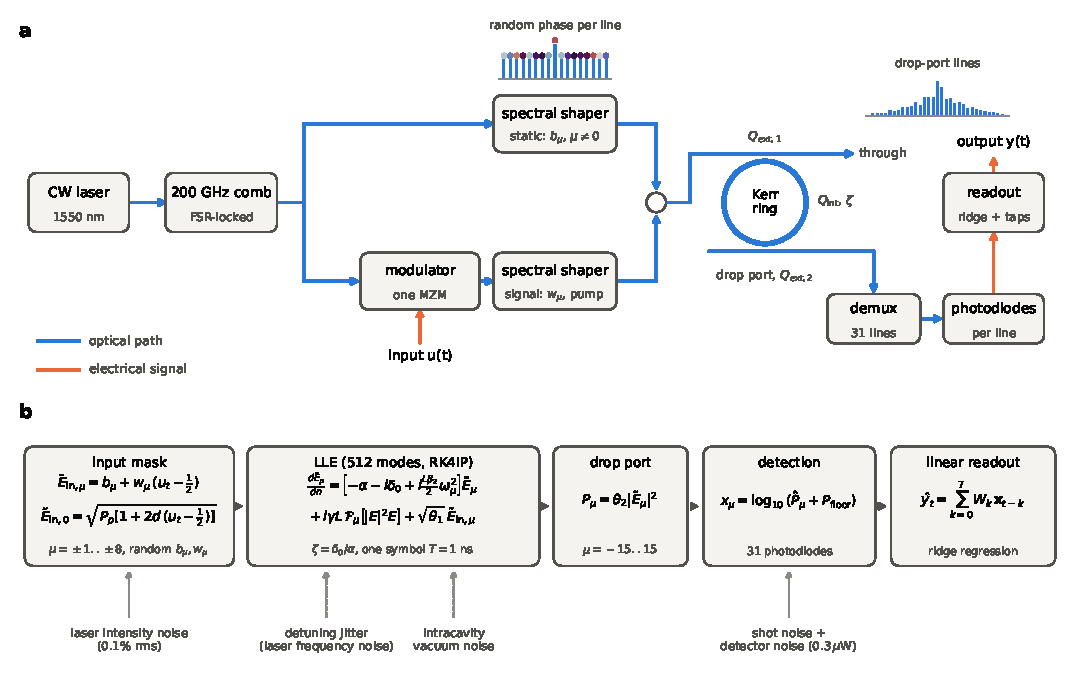
\includegraphics[width=\linewidth]{fig1_scheme}
\caption{Scheme and model.
(a) Optical layout. A $200~\mathrm{GHz}$ input comb locked to the resonator FSR is split in two: the static branch passes a
spectral phase shaper that writes the biases $b_\mu$; the other branch carries the signal $u(t)$ through one modulator and a
second shaper that writes the weights $w_\mu$. The recombined comb and the pump drive an add--drop Kerr ring (input coupling
$\Qone$, drop coupling $\Qtwo$, intrinsic $\Qint$, normalised detuning $\zeta$). The 31 drop-port lines are demultiplexed and
detected separately, and a ridge readout with delay taps combines them into the output $y(t)$. Insets: random phases of the input
lines (colour) and a sketch of the drop-port spectrum.
(b) Signal chain of the simulation model: input mask (Eq.~\eqref{eq:mask}), Lugiato--Lefever equation (Eq.~\eqref{eq:lle}),
drop-port power, logarithmic detection and linear readout; dashed arrows mark where the five noise sources enter
(Section~\ref{sec:noise-model}).}
\label{fig:scheme}
\end{figure}

The intracavity field is described by the mean-field Lugiato--Lefever equation (LLE)~\cite{lugiato1987,coen2013}.
With the round-trip number $n=t/t_R$ as slow time, the field amplitude $\tilde E_\mu$ of longitudinal mode $\mu$ (counted from the
pump), with angular frequency offset $\omega_\mu=2\pi\,\mathrm{FSR}\,\mu$, obeys
\begin{equation}
\frac{\mathrm d\tilde E_\mu}{\mathrm dn}
=\Big[-\alpha-i\delta_0+i\frac{L\beta_2}{2}\,\omega_\mu^{2}\Big]\tilde E_\mu
+i\gamma L\,\mathcal F_\mu\!\big[|E|^{2}E\big]
+\sqrt{\theta_1}\,\tilde E_{\mathrm{in},\mu}(u_t),
\label{eq:lle}
\end{equation}
where $E(\tau)$ is the intracavity field on the fast-time grid ($|E|^2$ in watts), $\mathcal F_\mu$ takes the $\mu$-th Fourier
component, $\theta_1$ and $\theta_2$ are the power coupling ratios of the two ports, $\alpha=(\alpha_i+\theta_1+\theta_2)/2$ is
the field loss per round trip (the half-linewidth), and $\delta_0$ is the pump detuning from resonance. We use the normalised
detuning $\zeta=\delta_0/\alpha$ (in half-linewidths), drawn in $[-1,4]$ for each operating point.
The loaded quality factor is $Q=\omega_0 t_R/(2\alpha)$, and the drop-port power of line $\mu$ is $P_\mu=\theta_2|\tilde E_\mu|^{2}$.

Equation~\eqref{eq:lle} is integrated with the fourth-order Runge--Kutta method in the interaction picture
(RK4IP)~\cite{hult2007}, which uses only fast Fourier transforms and pointwise operations, so gradients with respect to all device
parameters are available (Section~\ref{sec:gradient}).
By default we use 512 modes and 20 steps per $1~\mathrm{ns}$ symbol (about 200 round trips).
Results agree between 512 and 1024 modes (Appendix~\ref{app:checks}).

\subsection{Input encodings}\label{sec:encodings-def}

The input is a sequence of symbols $u_t\in[0,1]$, each held for $T=1~\mathrm{ns}$. We compare eight ways of feeding $u_t$ into the
resonator.

\paragraph{Spectral-phase input mask (this work).}
The input field consists of the pump ($\mu=0$) and eight input lines on each side ($\mu=\pm1,\dots,\pm8$):
\begin{equation}
\tilde E_{\mathrm{in},0}=\sqrt{P_p\,[1+2d\,(u_t-\tfrac12)]},\qquad
\tilde E_{\mathrm{in},\mu}=b_\mu+w_\mu\,(u_t-\tfrac12)\quad(\mu=\pm1,\dots,\pm8).
\label{eq:mask}
\end{equation}
The bias $b_\mu$ and modulation weight $w_\mu$ of every line are independent complex Gaussian numbers, i.e.\ random amplitudes and
random phases. They are scaled together so that the mean sideband power $\sum_\mu\big(|b_\mu|^{2}+|w_\mu|^{2}/12\big)$ is a fraction
$f_s$ of the total power $P$, and the pump power is $P_p=(1-f_s)P$.
The random parameters of an operating point are the total power $P$ ($10$ to $300~\mathrm{mW}$, log-uniform), $f_s\in[0.1,0.9]$,
the modulation depth $d\in[0.05,0.9]$, $\zeta$ and $\Qone$.
Experimentally this corresponds to splitting an input comb into a static branch (giving $b_\mu$) and a branch through one modulator
(giving $w_\mu$), each passing a programmable spectral shaper before recombination. The ablation of Section~\ref{sec:ablation}
shows that what matters is the randomness of the line phases, so the shapers need only set phases.

\paragraph{Single-pump encodings (literature schemes).}
A single CW pump whose power $P[1+d(u_t-\tfrac12)]$~\cite{shishavan2025}, detuning $\zeta+d(u_t-\tfrac12)$~\cite{cuevas2025} or
phase $\exp[i d(u_t-\tfrac12)]$~\cite{arabieh2026soliton} is modulated by the signal.
The power encoding uses $d\in[0.05,1]$; the detuning and phase encodings draw $d$ log-uniformly between $10^{-1.3}$ and $10^{0.5}$.
Each comes in two groups: the cavity starts from an empty field, or from a single soliton (the soliton groups draw $\zeta$ inside
the soliton existence range, $\Qone\in[10^{6.5},10^{7.2}]$ and $P\in[30,300]~\mathrm{mW}$).

\paragraph{Uniformly modulated comb.}
The same 16 input lines as the mask, but with equal amplitudes and equal phases, all modulated together by the same signal, which
corresponds to a modulated synchronous pulse train~\cite{arabieh2026pulse}.

All encodings use the same device, the same power and $Q$ ranges and the same readout, and draw the same number of random
operating points (Section~\ref{sec:protocol}).

\subsection{Readout}\label{sec:readout-def}

The central 31 lines of the drop port ($\mu=-15,\dots,15$) are demultiplexed and detected by separate photodiodes.
The readings are log-compressed, $x_\mu=\log_{10}(\hat P_\mu+P_\mathrm{floor})$, where $\hat P_\mu$ is the noisy reading and
$P_\mathrm{floor}$ the larger of the detector noise and $1~\mathrm{nW}$, so that dark lines do not dominate the regression after
the logarithm. Besides the 31 readings of the current symbol the readout sees those of the previous seven symbols (8 delay taps,
248 features; 12 taps for NARMA-10) and is a ridge regression on standardised features, with the regularisation chosen on the
validation part from $\{10^{-8},10^{-6},10^{-4},10^{-2},1\}$. Section~\ref{sec:memory} discusses the memory these taps provide.

\subsection{Noise model}\label{sec:noise-model}

``Realistic noise'' has three sources inside the device and two at detection:
\begin{itemize}
\item laser intensity noise: $0.1\%$ relative rms, one sample per symbol, shared by the pump and all input lines;
\item detuning jitter: the pump detuning from resonance fluctuates by $1\%$ of the half-linewidth (rms) per symbol, with a
      correlation time of one symbol; for white frequency noise this corresponds to a laser with an intrinsic linewidth of about
      $1.6~\mathrm{kHz}$ (Section~\ref{sec:laser} checks this against real laser frequency-noise spectra);
\item intracavity field noise at the vacuum level: half a photon per mode and loss channel;
\item shot noise, with each reading integrated over one symbol ($1~\mathrm{ns}$);
\item detector electronic noise of $0.3~\mu\mathrm{W}$ per line (rms, referred to optical power). For 1-GHz-class InGaAs PIN
      receivers the datasheet noise-equivalent power corresponds to $0.13$ to $0.63~\mu\mathrm{W}$ per line, so $0.3~\mu\mathrm{W}$
      is mid-range.
\end{itemize}
Amplified-spontaneous-emission beat noise and detector quantum efficiency are not modelled. Section~\ref{sec:noise} breaks down
the contribution of each source.

\subsection{Tasks and software baselines}\label{sec:tasks}

Three benchmark tasks:
(1) ten-step prediction of the Mackey--Glass series ($\tau=17$, $\beta=0.2$, $\gamma=0.1$, exponent 10, sampling interval 1);
(2) nonlinear channel equalisation~\cite{jaeger2004}: four-level symbols pass linear inter-symbol interference, a cubic
polynomial nonlinearity and additive noise at $28~\mathrm{dB}$ SNR, and the symbol sent two steps earlier is recovered from the
received signal (we report the symbol error rate besides the NMSE);
(3) NARMA-10, which needs a memory of about ten symbols.
Appendix~\ref{app:fibre} adds a realistic fibre-link task (28~GBd PAM-4 over 17~km of standard single-mode fibre, intensity
modulation and direct detection).

There are two software baselines. One is an echo state network (ESN)~\cite{jaeger2001} with 31 $\tanh$ nodes, matching the
resonator's readout dimension, whose readout sees the same delay taps and whose spectral radius and input scaling are chosen on the
validation part; Section~\ref{sec:software} adds ESNs of 100 to 1000 nodes and next-generation reservoir computing
(NG-RC)~\cite{gauthier2021}. The other is linear autoregression with up to 32 lagged inputs.
Under realistic noise the baselines receive input noise of $3\times10^{-3}$ rms, i.e.\ the laser intensity noise referred to the
input through a modulation depth of $0.33$; this convention strongly affects the comparison, and Section~\ref{sec:software} gives
the full sweep.

\subsection{Evaluation protocol}\label{sec:protocol}

Each series discards 300 warm-up symbols and then uses 1700 symbols, split 60/20/20 into training, validation and test parts (for
channel equalisation under realistic noise the test part is extended to 5000 symbols to resolve the symbol error rate).
Errors are normalised mean-square errors (NMSE). A physical device never sees the same noise twice, so the readout is always
trained on one run and tested on another run with independent noise (cross-run NMSE).

Operating points are chosen in two steps, so that a point that was merely lucky is not picked: for each encoding we draw 256
random operating points, run each once (a pair of runs) and keep the 16 best on validation error; these 16 are run on three new
pairs, and the one with the lowest mean validation error is chosen; we report its mean test error on six further new pairs.
Every setting is repeated on three independent series and the geometric mean is reported.
Choosing and reporting on a single noise realisation would be optimistic by 10 to 30\% (Appendix~\ref{app:checks}).

\section{Coherently seeded regime: why the output is reproducible}\label{sec:mechanism}

Reservoir computing requires that the same input gives the same output; otherwise a trained readout fails on the next run.
In the single-pump schemes of the literature the comb lines either grow out of noise through modulation
instability~\cite{shishavan2025} or rely on a soliton state prepared beforehand~\cite{cuevas2025,arabieh2026soliton}.
The former's output depends on the noise at start-up; the latter needs the device to be held inside the soliton existence range.
The spectral-phase mask gives a third mode of operation: the input lines themselves sit on resonances and the sidebands are
seeded coherently by the input instead of growing from noise, so the output is set by the input.

\subsection{Two runs compared}

Figure~\ref{fig:two-runs} feeds the same input sequence into the same device twice; the two runs differ only in the initial
intracavity noise. Panel~(a) uses the parameters of the original chaotic-comb scheme (a single CW pump, $325~\mathrm{mW}$, loaded
$Q=10^{7}$, normalised detuning about 5): the power of the third line next to the pump is completely different in the two runs, with
a correlation of only $0.08$; a readout trained on such features gives an NMSE of about 1 on the other run, i.e.\ it learned
nothing. Panel~(b) is an operating point of the spectral-phase mask (the point chosen in the noise-floor study of
Section~\ref{sec:noise}, $23~\mathrm{mW}$, loaded $Q=6\times10^{6}$): the two curves coincide, with correlation $1.00$.

\begin{figure}[htbp]
\centering
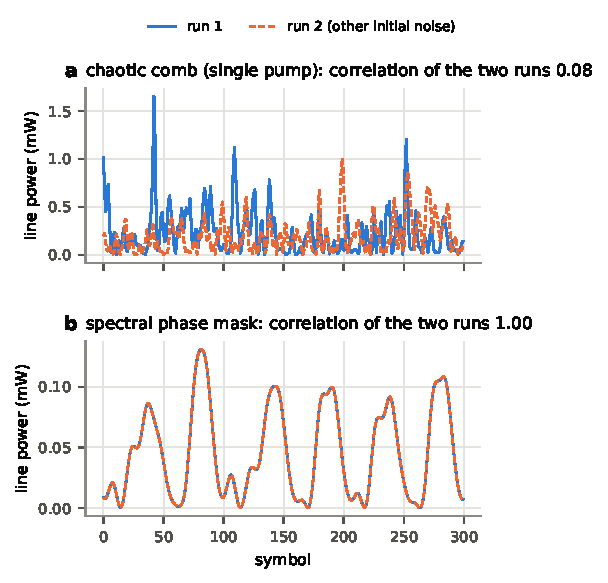
\includegraphics[width=0.8\linewidth]{fig3_two_runs}
\caption{The same input sequence fed into the same device twice; the runs differ only in the initial intracavity noise (solid and
dashed). Shown is the drop-port power of the third line next to the pump over the first 300 symbols.
(a) Parameters of the original chaotic-comb scheme (single CW pump, $325~\mathrm{mW}$, loaded $Q=10^{7}$, normalised detuning
about 5): correlation between the runs $0.08$.
(b) An operating point of the spectral-phase mask ($23~\mathrm{mW}$, loaded $Q=6\times10^{6}$): the curves coincide, correlation
$1.00$. No other noise in either panel.}
\label{fig:two-runs}
\end{figure}

\subsection{Operating map}

Reproducibility holds only in part of the parameter space. Figure~\ref{fig:operating-map} fixes the other parameters of a mask
operating point and scans only the input coupling $\Qone$ ($10^{5.6}$ to $10^{7.6}$) and the total input power ($3$ to
$1000~\mathrm{mW}$) in 17 steps each, plotting the Mackey--Glass test error; for every point we also compute the consistency of
two runs (the correlation between their features).

Without noise the plane splits in two. 74\% of the points have a consistency above $0.99$: the coherently seeded regime.
The inconsistent points (consistency below $0.5$, 16\%) gather in the high-power, high-$Q$ corner (above $163~\mathrm{mW}$), where
the intracavity power lets modulation instability overwhelm the seed and the comb returns to chaos.
The lowest errors lie inside the coherently seeded regime, close to the chaotic one: all points within a factor of three of the
best error ($1.8\times10^{-6}$) fall between $6$ and $79~\mathrm{mW}$ and $\Qone=10^{6.1}$ to $10^{6.85}$. This matches the common
experience in reservoir computing that more nonlinearity helps, but not so much that reproducibility is lost.

Realistic noise adds a third region. At low power many lines reach the detectors with powers comparable to the detector noise,
the readings drown in it, and the consistency drops as well; the share of points with consistency above $0.99$ falls from 74\% to
29\%. The usable operating points are squeezed between the two: limited by detector noise on the low-power side and by chaos on
the high-power side, the points within a factor of three of the best error ($3.3\times10^{-4}$) form a diagonal band in the
power--$Q$ plane ($9$ to $336~\mathrm{mW}$). The higher the $Q$, the less power is needed for the same nonlinearity, so the band
tilts towards lower power as $Q$ increases. The chaotic region is at the same place with and without noise, because its cause
(modulation-instability gain exceeding the seed) does not depend on the noise.

\begin{figure}[htbp]
\centering
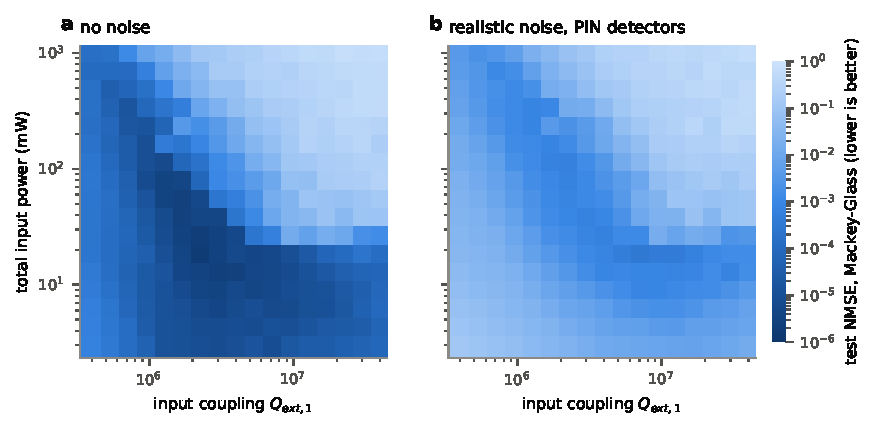
\includegraphics[width=\linewidth]{fig2_operating_map}
\caption{Operating map of the spectral-phase mask. The other parameters of a mask operating point are fixed while the input
coupling $\Qone$ and the total input power are scanned (17 steps each); colour is the Mackey--Glass test error (darker is better).
(a) No noise: the upper right (high power, high $Q$) is the non-reproducible chaotic regime, the rest is coherently seeded, and the
lowest errors lie in the seeded regime close to the chaotic one.
(b) Realistic noise, PIN detectors: the low-power region drowns in detector noise, and the usable points form a band between the
two regions that tilts towards lower power as $Q$ increases. The run-to-run consistency values are given in the text.}
\label{fig:operating-map}
\end{figure}

The conclusion of this section is used throughout the rest of the paper: the spectral-phase mask operates in the coherently seeded
regime, and its error comes from noise, not from non-reproducible dynamics. Lowering the error therefore requires knowing which
noise source is responsible (Section~\ref{sec:noise}).

\section{Comparison of encodings}\label{sec:encodings}

This section compares eight encodings under identical physical conditions: the same simulator, the same device-parameter and
optical-power ranges, the same readout (31 lines, 8 taps), the same noise model, and the same number of random operating points
with the same selection procedure (Section~\ref{sec:protocol}). Table~\ref{tab:encodings} summarises the three tasks with and
without noise, and Fig.~\ref{fig:encodings} plots the same numbers.

% generated by experiments/make_table1.py; do not edit by hand
\begin{table*}[htbp]
\centering
\caption{Test error (NMSE, lower is better) of each encoding and the baselines. Each encoding draws 256 random operating points over the same ranges; the point is chosen on the mean validation error of new runs and the mean test error over six further pairs of new runs is reported, as the geometric mean over three series; the readout is trained on one run and tested on another with independent noise. The best resonator encoding in each column is in bold. The ESN has the same readout dimension as the resonator (31 nodes, the same delay taps) and uses a single random reservoir; under realistic noise its input noise is $3\times10^{-3}$; stronger software baselines are in Section~\ref{sec:software}. Channel equalisation under realistic noise uses test parts of 5000 symbols.}
\label{tab:encodings}
\footnotesize\setlength{\tabcolsep}{4pt}
\begin{tabular}{lcccccc}
\toprule
 & \multicolumn{2}{c}{Mackey--Glass (10 steps)} & \multicolumn{2}{c}{channel equalisation} & \multicolumn{2}{c}{NARMA-10} \\
\cmidrule(lr){2-3}\cmidrule(lr){4-5}\cmidrule(lr){6-7}
encoding & no noise & realistic & no noise & realistic & no noise & realistic \\
\midrule
pump power~\cite{shishavan2025} & $0.20$ & $0.33$ & $7.6\times10^{-3}$ & $1.0\times10^{-2}$ & $0.21$ & $0.35$ \\
pump detuning~\cite{cuevas2025} & $5.6\times10^{-2}$ & $9.3\times10^{-2}$ & $1.2\times10^{-2}$ & $3.0\times10^{-2}$ & $0.21$ & $0.45$ \\
pump phase~\cite{arabieh2026soliton} & $0.14$ & $0.20$ & $4.8\times10^{-2}$ & $7.7\times10^{-2}$ & $0.66$ & $1.0$ \\
pump power, soliton start & $1.9\times10^{-3}$ & $5.3\times10^{-2}$ & $1.1\times10^{-2}$ & $2.1\times10^{-2}$ & $0.20$ & $0.32$ \\
pump detuning, soliton start & $1.7\times10^{-3}$ & $9.5\times10^{-2}$ & $1.2\times10^{-2}$ & $0.17$ & $0.19$ & $0.39$ \\
pump phase, soliton start & $2.8\times10^{-3}$ & $5.0\times10^{-2}$ & $3.5\times10^{-2}$ & $6.0\times10^{-2}$ & $0.68$ & $0.74$ \\
uniformly modulated comb & $8.2\times10^{-5}$ & $4.8\times10^{-3}$ & $5.0\times10^{-3}$ & $7.6\times10^{-3}$ & $0.18$ & $0.21$ \\
spectral-phase mask (this work) & $\mathbf{1.8\times10^{-6}}$ & $\mathbf{3.3\times10^{-4}}$ & $\mathbf{3.7\times10^{-3}}$ & $\mathbf{5.7\times10^{-3}}$ & $\mathbf{0.16}$ & $\mathbf{0.19}$ \\
\midrule
ESN (31 nodes) & $2.4\times10^{-5}$ & $3.2\times10^{-4}$ & $3.8\times10^{-3}$ & $4.0\times10^{-3}$ & $0.11$ & $0.11$ \\
linear autoregression & $0.14$ & $0.21$ & $1.1\times10^{-2}$ & $1.3\times10^{-2}$ & $0.19$ & $0.19$ \\
\bottomrule
\end{tabular}
\end{table*}


\begin{figure}[htbp]
\centering
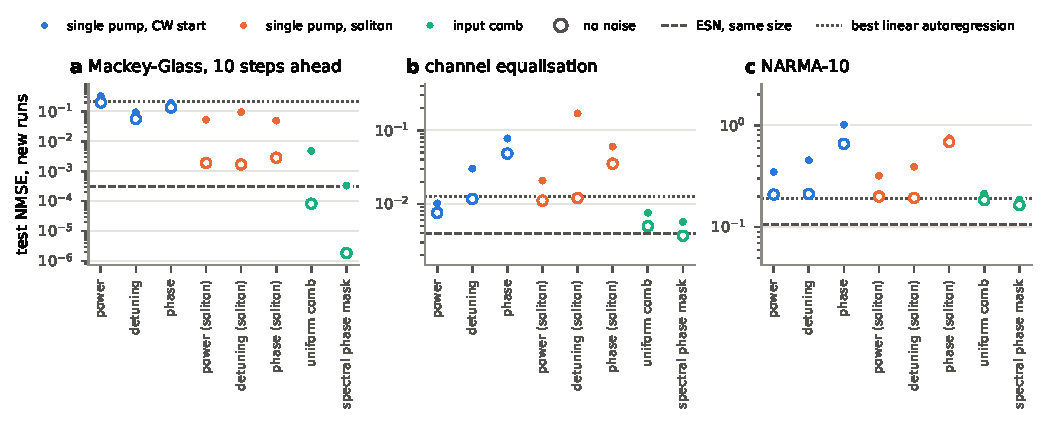
\includegraphics[width=\linewidth]{fig4_encodings}
\caption{Test error of the eight encodings on the three tasks under realistic noise (the ``realistic noise'' columns of
Table~\ref{tab:encodings}; new runs, geometric mean over three series).
Blue: single-pump encodings starting from an empty cavity; orange: single-pump encodings starting from a single soliton; green:
input combs (uniform modulation and spectral-phase mask). Dashed: ESN with the same readout dimension (input noise
$3\times10^{-3}$); dotted: best linear autoregression.
(a) Mackey--Glass, ten steps ahead; (b) nonlinear channel equalisation; (c) NARMA-10.}
\label{fig:encodings}
\end{figure}

\subsection{Mackey--Glass prediction}

The spectral-phase mask has its largest advantage on Mackey--Glass. Without noise its test error is $1.8\times10^{-6}$, about 45
times better than the uniformly modulated comb ($8.2\times10^{-5}$), about 900 times better than the best single-pump encoding
(detuning, soliton start, $1.7\times10^{-3}$), and four to five orders of magnitude better than single-pump encodings starting
from an empty cavity. Under realistic noise every encoding degrades but the order stays: the mask reaches $3.3\times10^{-4}$, the
uniform comb $4.8\times10^{-3}$ (about 15 times worse) and the best single-pump encoding $5.0\times10^{-2}$ (about 150 times
worse).

The ESN with the same readout dimension reaches $2.4\times10^{-5}$ without noise, 13 times worse than the mask; under realistic
noise it reaches $3.2\times10^{-4}$, on par with the mask. The latter comparison depends on the input noise given to the ESN
($3\times10^{-3}$ here) and on using a single random reservoir: with several reservoirs the ESN reaches $1.9\times10^{-4}$, and with
input noise $10^{-3}$ it reaches $5.3\times10^{-5}$. Section~\ref{sec:software} is devoted to this comparison; this section only
compares optical encodings, which share one noise model and are not affected by the convention.

\subsection{The advantage does not come from one lucky operating point}

The best result of an encoding might just be one particularly good draw out of 256. Figure~\ref{fig:distributions} shows the error
distribution over all random operating points of each encoding (Mackey--Glass under realistic noise, 768 points over three series).
The whole distribution of the mask is shifted: its median, $4.3\times10^{-2}$, is already better than the best 10\% of every
single-pump encoding ($0.14$ to $0.38$), and its best 10\% lie below $1.9\times10^{-3}$, more than an order of magnitude better than
the best 10\% of the uniform comb ($2.5\times10^{-2}$). The advantage is thus a property of this class of input, not of a
particular parameter combination.

\begin{figure}[htbp]
\centering
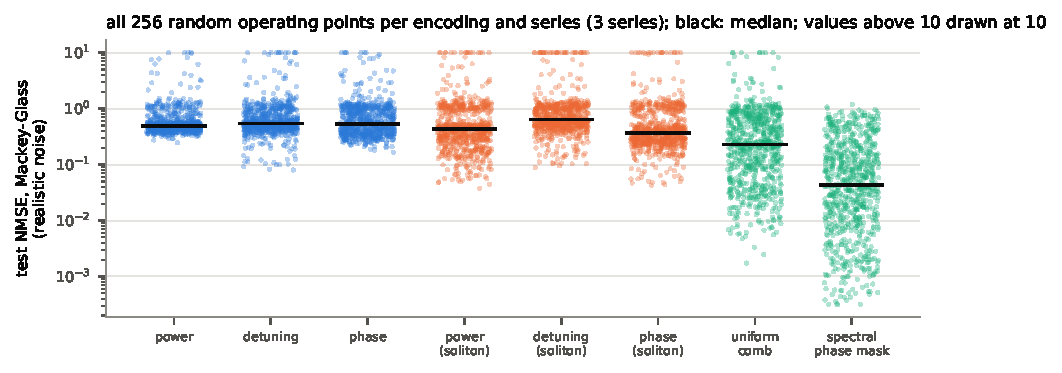
\includegraphics[width=\linewidth]{fig5_distributions}
\caption{Distribution of the Mackey--Glass test error under realistic noise: 256 random operating points per encoding and series
(768 points over three series, one pair of runs per point); black bars are medians, values above 10 are drawn at 10. Colours as in
Fig.~\ref{fig:encodings}.}
\label{fig:distributions}
\end{figure}

\subsection{Channel equalisation}

The differences are much smaller on channel equalisation. The mask is still the best optical encoding, $3.7\times10^{-3}$ without
noise and $5.7\times10^{-3}$ with realistic noise: about 1.3 times better than the uniform comb, about 2 times better than the best
single-pump encoding (power) and 2 to 3 times better than linear autoregression ($1.1\times10^{-2}$ and $1.3\times10^{-2}$).
Without noise the mask ties with the ESN ($3.8\times10^{-3}$); with realistic noise the ESN reaches $4.0\times10^{-3}$, about 1.4
times better than the mask. The error of this task comes mostly from the channel's own noise; Section~\ref{sec:software} shows that
removing the ESN's input noise entirely improves it by only about 7\%.
In symbol error rate (six new runs of 5000 test symbols per series, 90\,000 symbols over three series) the mask reaches
$1.9\times10^{-4}$ (17 errors), the uniform comb $1.0\times10^{-4}$ (9), the power encoding $3.9\times10^{-4}$ (35) and the ESN
$1.1\times10^{-5}$ (1). The mask and the uniform comb cannot be separated by this statistic; all comb encodings and the ESN are far
below the common hard-decision FEC threshold of $3.8\times10^{-3}$.

\subsection{NARMA-10: where a single ring does not work}

NARMA-10 needs a memory of about ten symbols, whereas the resonator's own memory is its photon lifetime, a few symbols at most.
With a single resonator the mask ($0.16$ without noise, $0.19$ with realistic noise) only ties with linear autoregression ($0.19$),
slightly better than the uniform comb and the single-pump encodings but 1.5 to 1.8 times worse than the ESN ($0.11$). We report this
as a negative case. Memory can be added from outside: with a delayed copy of the signal on the input lines (an input delay line)
and several rings with different masks read out together, NARMA-10 drops to $0.011$, on par with a 100-node ESN with the same delay
line ($0.010$; Section~\ref{sec:memory}).

\subsection{What matters is the randomness of the line phases}\label{sec:ablation}

To find out which part of the mask matters, we compared simplified masks over the same operating-point ranges (realistic noise,
the protocol of Table~\ref{tab:encodings}, 128 points each; Appendix~\ref{app:ablation}). On Mackey--Glass:
\begin{itemize}
\item random phases with equal line amplitudes: $2.4\times10^{-4}$, as good as or slightly better than the full mask
      ($3.8\times10^{-4}$ in this set of runs);
\item random amplitudes with all lines in phase: $1.3\times10^{-3}$, 3 to 6 times worse;
\item a random static spectrum with one common modulation ($w_\mu\propto b_\mu$): $6.5\times10^{-4}$;
\item equal amplitudes and phases (uniform modulation): $5.0\times10^{-3}$.
\end{itemize}
Channel equalisation gives the same order with smaller differences (phases only $5.0\times10^{-3}$, full mask $5.4\times10^{-3}$,
amplitudes only $5.8\times10^{-3}$, uniform $7.3\times10^{-3}$).
The number of input lines matters too: on Mackey--Glass 4, 8, 16, 32 and 64 lines give $1.9\times10^{-3}$, $1.4\times10^{-3}$,
$3.8\times10^{-4}$, $2.4\times10^{-4}$ and $2.1\times10^{-4}$, with little further gain beyond 32; on channel equalisation 32 lines
are best ($4.0\times10^{-3}$) and 64 are worse ($5.6\times10^{-3}$).

This gives the first design rule: \emph{what matters is the randomness of the line phases, not independent amplitude modulation of
each line}. No per-line modulators are needed; one modulator and two phase-only spectral shapers suffice.
We do not yet have a complete explanation of why phases matter more than amplitudes. An intuitive guess is that random phases make
the four-wave-mixing paths from different input lines into a given output line interfere differently, so that the line features are
less correlated with each other. At the linear level this guess fails. At the operating point chosen for each variant (no noise,
Mackey--Glass) we computed the correlation matrix of the 31 line features: the effective rank (participation ratio, the squared sum
of the eigenvalues divided by the sum of their squares) is $2.2$, $2.3$, $2.4$, $2.2$ and $2.0$ for the uniform comb, the random
spectrum with common modulation, amplitudes only, phases only and the full mask, and the mean absolute correlation is $0.58$,
$0.58$, $0.57$, $0.60$ and $0.65$. The variants are nearly identical, and the full mask even has the lowest linear diversity. The
benefit of the mask therefore does not lie in linear decorrelation of the instantaneous features; more likely the features are
different higher-order nonlinear functions of the input history. Testing this needs a decomposition such as the information
processing capacity and is left for future work.

\section{The noise floor}\label{sec:noise}

Realistic noise raises the Mackey--Glass error of the spectral-phase mask from $1.8\times10^{-6}$ to $3.3\times10^{-4}$, a factor of
about 180 (Table~\ref{tab:encodings}). Section~\ref{sec:mechanism} showed that the mask operates in the coherently seeded regime, so
its error comes from noise, not from non-reproducible dynamics. This section separates the five noise sources to answer three
questions: which of them set the floor; whether a more nonlinear material or more power lowers it; and whether it can be removed
in the readout. The answer: about half of the floor comes from detuning jitter and half from shot noise. The first half does not
depend on the photon number; the second falls with more photons, but then the first half quickly dominates, so neither
Si$_3$N$_4$ nor more power helps much. A linear readout cannot remove the jitter even when it knows the exact jitter sequence, so it
has to be suppressed at the source, which sets a requirement on the laser linewidth.

\subsection{Breakdown}\label{sec:breakdown}

To separate the detectors from the noise inside the device, we first assume ideal detectors (no electronic noise, shot noise only),
choose the best of 256 random operating points with the protocol of Section~\ref{sec:protocol}, and switch on one noise source at a
time at that point (Fig.~\ref{fig:noise}a). The point uses $23~\mathrm{mW}$ in total, a loaded $Q$ of $6\times10^{6}$, and about
$170~\mu\mathrm{W}$ per line at the detector, i.e.\ about $1.3\times10^{6}$ photons per symbol.
Its error without noise is $1.3\times10^{-5}$. With only the laser intensity noise it is $1.9\times10^{-5}$, nearly unchanged; with
only the intracavity vacuum noise $2.5\times10^{-5}$; with only the detuning jitter $5.7\times10^{-5}$; with only shot noise
$6.8\times10^{-5}$. The three optical sources together give $7.8\times10^{-5}$, and adding shot noise gives $1.5\times10^{-4}$.
The floor with ideal detectors is therefore about $1.3\times10^{-4}$ (after re-selecting among 256 points), about half from
detuning jitter and half from shot noise, with the vacuum noise secondary and the laser intensity noise negligible.

With realistic PIN detectors ($0.3~\mu\mathrm{W}$ electronic noise per line) the same procedure selects a point at
$3.4\times10^{-4}$, another factor of about 2.5. The effect of the detectors shows most clearly in an earlier, smaller search (32
candidates per encoding, selection on a single run): with all noise on and detector noise of $0.03$, $0.1$, $0.3$ and
$0.6~\mu\mathrm{W}$ the error is $2.7\times10^{-4}$, $4.1\times10^{-4}$, $1.0\times10^{-3}$ and $2.2\times10^{-3}$, roughly linear in
the detector noise above $0.1~\mu\mathrm{W}$; an optical amplifier with $10~\mathrm{dB}$ or $20~\mathrm{dB}$ gain and a
$5~\mathrm{dB}$ noise figure in front of the $0.3~\mu\mathrm{W}$ detectors brings it to $3.3\times10^{-4}$ and $3.1\times10^{-4}$,
close to the $2.4\times10^{-4}$ with optical and shot noise only. These numbers cannot be compared directly with
Table~\ref{tab:encodings} (fewer candidates, different selection); we use them only for the trend: electronic detector noise can be
removed with an optical amplifier, and what remains is the floor above.

\begin{figure}[htbp]
\centering
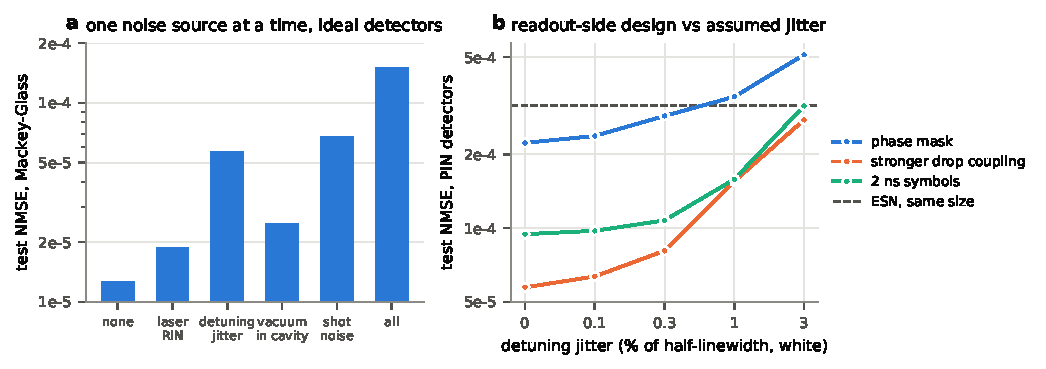
\includegraphics[width=\linewidth]{fig6_noise}
\caption{Noise and readout-side design (Mackey--Glass).
(a) Test error at the best of 256 operating points with ideal detectors, one noise source at a time; ``all'' has the four sources
(laser intensity noise, detuning jitter, intracavity vacuum noise, shot noise) on together.
(b) Test error, with the operating point re-selected at each level, against the assumed detuning jitter (rms per symbol in percent
of the half-linewidth, correlation $e^{-1}$ between neighbouring symbols; the horizontal axis is categorical), PIN detectors: plain
spectral-phase mask, stronger drop coupling, $2~\mathrm{ns}$ symbols; dashed: ESN with the same readout dimension (input noise
$3\times10^{-3}$, one random reservoir). The top axis gives the intrinsic laser linewidth that produces the same jitter at the
stronger-drop-coupling point ($Q=1.9\times10^{6}$, $1~\mathrm{ns}$, Eq.~\eqref{eq:linewidth}); for the $2~\mathrm{ns}$ point
($Q=5\times10^{6}$) the linewidths are about 0.3 times these.}
\label{fig:noise}
\end{figure}

\subsection{Neither a more nonlinear material nor more power lowers the floor}\label{sec:platform}

Shot noise can be reduced with more photons; detuning jitter cannot, because it is defined relative to the resonance linewidth and
does not depend on how many photons are in the cavity. We changed the photon number in two ways, re-searching 256 operating points
each time (ideal detectors):
\begin{itemize}
\item a Si$_3$N$_4$ ring (nonlinear coefficient about 60 times that of silica, power range scaled with $\gamma L$ so that the
      normalised pump covers the same range): the best point needs only $5~\mathrm{mW}$ and delivers about 8 times fewer photons to
      the detectors, yet the floor is $1.4\times10^{-4}$, the same as silica's $1.3\times10^{-4}$;
\item a silica ring with ten times the power range ($0.1$ to $3~\mathrm{W}$): the floor is $1.5\times10^{-4}$, no improvement. Its best
      point has 4.4 times more photons per line than the point above, but the shot-noise term only falls from $6.8\times10^{-5}$ to
      $5.3\times10^{-5}$, and the jitter term ($5.1\times10^{-5}$) barely changes.
\end{itemize}
The shot-noise term falls much more slowly than the photon number grows, but the two best points also differ in other parameters,
so this is only a rough comparison. A controlled comparison keeps the operating point and the intracavity dynamics fixed and changes
only the number of photons detected per reading (the best single ring, ideal detectors, three series $\times$ six new pairs): with
1, 10 and 100 times the photons the total error is $1.41\times10^{-4}$, $1.21\times10^{-4}$ and $1.16\times10^{-4}$, and
$1.16\times10^{-4}$ without shot noise. The shot-noise term itself does fall with the photon number (about 5 times for 10 times the
photons, about 40 times for 100 times), but the total quickly settles at the level set by the optical noise, mostly detuning jitter.
At this point more power can lower the error by at most about 18\%.
The benefit of Si$_3$N$_4$ is power: the same floor needs about a quarter of the power; but with ordinary detectors fewer photons
reach them and the error rises to $1.1\times10^{-3}$, so it needs better detectors or an optical amplifier.
What does lower the floor is the readout side: stronger drop coupling (more light to the detectors) or $2~\mathrm{ns}$ symbols (longer
integration per reading) bring it to $8.7\times10^{-5}$ and $6.9\times10^{-5}$ with ideal detectors, and $1.55\times10^{-4}$ and
$1.58\times10^{-4}$ with ordinary detectors (Section~\ref{sec:readout}).

\subsection{A linear readout cannot remove the detuning jitter}\label{sec:reference}

If the detuning jitter comes mainly from the frequency noise of the pump laser, all rings on one chip driven by the same laser see
the same jitter. A natural idea is a reference ring without signal that measures this common-mode noise so the readout can subtract
it. We first measure the upper bound of this idea: on the best single ring (stronger drop coupling, $Q=1.9\times10^{6}$,
$178~\mathrm{mW}$) we hand the readout the true jitter sequence of each run (current and previous seven symbols), i.e.\ a noiseless
ideal reference. Over three series with six new pairs each, the plain readout gives $1.60\times10^{-4}$; adding the true jitter
sequence gives $1.58\times10^{-4}$, only 2\% better; also adding the products of the current jitter with the line features (so that
the correction can depend on the state) is slightly worse, $1.65\times10^{-4}$. Switching the jitter itself off, with all other
noise unchanged, gives $5.7\times10^{-5}$, 2.8 times better.

So the jitter is indeed the larger part of the floor, but even when it is known exactly a linear readout cannot remove it.
The reason is that the jitter is not additive noise on the readings: it changes the intracavity detuning, which changes the state of
the whole comb through the nonlinear dynamics and persists over the following symbols; its effect on each line depends on the state
at the time and cannot be subtracted linearly by the readout. A shared reference ring read out linearly therefore does not work. We
did not test nonlinear readouts, or feeding the reference ring's own 31 line features (which are nonlinear functions of the jitter
history) to the readout; these could recover part of the gap, but the jitter is most simply suppressed physically.

\subsection{Requirement on the intrinsic laser linewidth}\label{sec:laser}

The noise model above gives every symbol a detuning jitter of 1\% of the half-linewidth (rms). We now relate it to the laser.
For white frequency noise with Lorentzian linewidth $\Delta\nu$ (one-sided frequency-noise spectrum $S_\nu=\Delta\nu/\pi$), the
variance of the frequency averaged over a symbol time $T$ is $\Delta\nu/(2\pi T)$. In units of the half-linewidth $\nu/(2Q)$, the
relative jitter per symbol $\varepsilon$ and the linewidth are related by
\begin{equation}
\Delta\nu=2\pi T\left(\frac{\varepsilon\,\nu}{2Q}\right)^{2}.
\label{eq:linewidth}
\end{equation}
For the best single ring ($Q=1.9\times10^{6}$, half-linewidth $51~\mathrm{MHz}$, $T=1~\mathrm{ns}$), 1\% jitter corresponds to an
intrinsic linewidth of about $1.6~\mathrm{kHz}$, and 0.3\% and 0.1\% to about $150~\mathrm{Hz}$ and $16~\mathrm{Hz}$; conversely, a
laser with a $100~\mathrm{kHz}$ intrinsic linewidth produces about 8\% jitter. The required linewidth tightens with the square of $Q$
and relaxes with the symbol time: at the $2~\mathrm{ns}$ point of Section~\ref{sec:readout} ($Q=5\times10^{6}$), 1\% corresponds to
about $470~\mathrm{Hz}$.

To test this conversion we generate the jitter directly from a realistic laser frequency-noise spectrum $S_\nu(f)=h_0+h_{-1}/f$, where
$h_0=\Delta\nu/\pi$ is the white frequency noise and $h_{-1}/f$ the flicker noise (semiconductor lasers typically have a corner near
$1~\mathrm{MHz}$); the laser is locked to the resonance, and the suppression by the lock is modelled by a first-order high-pass
$f^{2}/(f^{2}+B^{2})$. A time series is synthesised from the spectrum, averaged within each symbol and divided by the half-linewidth to
give the jitter of each run; all other noise is unchanged. Table~\ref{tab:laser} gives the results.

% generated by experiments/make_table2.py; do not edit by hand
\begin{table}[htbp]
\centering
\caption{The best single ring under real lasers (stronger drop coupling, Mackey--Glass, all other realistic noise unchanged). The detuning jitter is the laser's white frequency noise averaged over each symbol. ``Fixed point'' is the point chosen under the 1\% jitter assumption ($Q=1.9\times10^{6}$); ``re-selected'' repeats the selection of Section~\ref{sec:protocol} under this laser's noise (56 candidates per series binned by $Q$). Three series $\times$ six new pairs. The two columns use different noise realisations; the same point differs by about 9\% between them.}
\label{tab:laser}
\small
\begin{tabular}{p{4.2cm}cccc}
\toprule
intrinsic linewidth & jitter/symbol & fixed point & re-selected & re-selected $Q$ \\
\midrule
100~Hz & 0.25\% & $6.7\times10^{-5}$ & -- & -- \\
1.6~kHz & 1.00\% & $1.3\times10^{-4}$ & $1.2\times10^{-4}$ & $1.9\times10^{6}$ \\
16~kHz & 3.15\% & $3.1\times10^{-4}$ & $2.9\times10^{-4}$ & $1.9\times10^{6}$ \\
100~kHz & 7.88\% & $8.1\times10^{-4}$ & $6.4\times10^{-4}$ & $1.9\times10^{6}$, $2.5\times10^{6}$ \\
1~MHz & 24.92\% & $5.2\times10^{-3}$ & $1.6\times10^{-3}$ & $1.2\times10^{6}$ \\
\midrule
100~kHz, flicker noise (1~MHz corner) and 1~MHz lock & 7.92\% & $8.3\times10^{-4}$ & -- & -- \\
1.6~kHz, flicker noise (10~MHz corner), no lock & 1.10\% & $1.8\times10^{-4}$ & -- & -- \\
\bottomrule
\end{tabular}
\end{table}


Table~\ref{tab:laser} shows four things. First, at nanosecond symbols what matters is the intrinsic (white-noise) linewidth: a
$1~\mathrm{ns}$ symbol corresponds to a bandwidth of about $500~\mathrm{MHz}$, almost entirely occupied by white frequency noise,
while the flicker noise is concentrated at low frequencies; adding flicker noise with a $1~\mathrm{MHz}$ corner and a
$1~\mathrm{MHz}$ lock leaves the $100~\mathrm{kHz}$ row nearly unchanged, and only very strong flicker noise ($10~\mathrm{MHz}$
corner) without any lock moves the $1.6~\mathrm{kHz}$ row from $1.3\times10^{-4}$ to $1.8\times10^{-4}$.
Second, our 1\% jitter model (correlation $e^{-1}$ between neighbouring symbols) gives $1.60\times10^{-4}$ at this point, about 25\%
more pessimistic than white frequency noise of the same rms ($1.27\times10^{-4}$), so at this point the main results are slightly
conservative. (The same point evaluated with other noise realisations gives $1.5$ to $1.6\times10^{-4}$; we use $1.55\times10^{-4}$
from Section~\ref{sec:readout} as its reference value.)
Third, changing the operating point does not avoid the requirement: at $1.6~\mathrm{kHz}$ and $16~\mathrm{kHz}$ re-selection returns
the original point; at $100~\mathrm{kHz}$ two series move to a point with $Q=2.5\times10^{6}$ and the error improves by about 1.3
times, more than the 9\% spread of one point between noise realisations but still modest; only at $1~\mathrm{MHz}$ does the choice
move clearly to lower $Q$ ($1.2\times10^{6}$), improving the error 3.3 times, yet the lowest $Q$ among the candidates (about
$5\times10^{5}$) is never chosen, because low-$Q$ points have weak nonlinearity and memory, which cancels the benefit of smaller
jitter.
Fourth, the position relative to software: the 31-node ESN with the same readout dimension and input noise $3\times10^{-3}$ reaches
$1.9\times10^{-4}$ (three reservoirs) to $3.2\times10^{-4}$ (one reservoir); by log interpolation of Table~\ref{tab:laser} the
intrinsic linewidth must be below about $5$ to $17~\mathrm{kHz}$ for the best single ring not to lose to it. Against
$1.9\times10^{-4}$, a $100~\mathrm{kHz}$ laser makes the ring about 4 times worse than the ESN, and a $1~\mathrm{MHz}$ laser about 8
times worse even after re-selection.

This gives the second design rule: \emph{half of the error floor is set by the laser's frequency noise relative to the resonance; a
linear readout cannot remove it and another operating point does not avoid it, so it calls for a narrow-linewidth source}.
For our device ($Q\sim2\times10^{6}$, $1~\mathrm{GBd}$) the intrinsic laser linewidth should be below a few kilohertz.
Self-injection locking of a laser to a microresonator is a known way to narrow semiconductor lasers by orders of
magnitude~\cite{shen2020,jin2021}: for example, self-injection locking an ordinary DFB laser to a silicon-nitride resonator with
$Q>2.6\times10^{8}$ suppresses its frequency noise by about five orders of magnitude and reaches a short-term linewidth of about
$1.2~\mathrm{Hz}$~\cite{jin2021}, far below the few kilohertz required here.
Thermorefractive noise of the ring itself is not included; it is mostly at low frequencies and is expected to matter little on
nanosecond scales after locking, but this needs a separate check.

\section{Readout-side design}\label{sec:readout}

Section~\ref{sec:noise} showed that neither another platform nor more power lowers the error floor with ideal detectors; only the
readout side and the light source can. This section presents two readout-side changes, how far they lower the error under realistic
noise and what they imply for the laser, and then asks where the readout's memory comes from.

\subsection{Stronger drop coupling and slower symbols}

The shot-noise half of the floor depends on the number of photons integrated per reading. There are two ways to increase it without
changing the intracavity dynamics:
\begin{itemize}
\item \emph{stronger drop coupling}: widen the range of $\Qtwo$ from a fixed $2.2\times10^{7}$ to $10^{6}$--$2.2\times10^{7}$, so that
      a larger fraction of the intracavity light leaves through the drop port to the detectors; the price is a lower loaded $Q$ and
      more power for the same nonlinearity;
\item \emph{slower symbols}: extend each symbol from $1~\mathrm{ns}$ to $2~\mathrm{ns}$, doubling the integration time per reading and
      giving the cavity more time to follow the input; the price is half the rate.
\end{itemize}
Both re-select among 256 random operating points with the protocol of Section~\ref{sec:protocol}. With ideal detectors they lower
the Mackey--Glass floor from $1.3\times10^{-4}$ to $8.7\times10^{-5}$ and $6.9\times10^{-5}$; with realistic noise (PIN detectors)
they reach $1.55\times10^{-4}$ and $1.58\times10^{-4}$, about 2 times better than the mask in Table~\ref{tab:encodings}
($3.3\times10^{-4}$). Stronger drop coupling selects a point with $Q=1.9\times10^{6}$ and $178~\mathrm{mW}$, the best single ring
used in Section~\ref{sec:reference} and Table~\ref{tab:laser}; slower symbols select a point with $Q=5\times10^{6}$.
Against the ESN with the same readout dimension, both tie with it or are slightly better when the ESN's input noise is
$3\times10^{-3}$ (the ESN reaches $1.9\times10^{-4}$ to $3.2\times10^{-4}$ depending on the random reservoir); below an input noise of
about $2.5\times10^{-3}$ the ESN is better (Section~\ref{sec:software}).

\subsection{Sensitivity to detuning jitter}

Both changes lower the shot-noise half; the other half (detuning jitter) is unaffected, so the improved error is more sensitive to
the jitter. Figure~\ref{fig:noise}b sweeps the assumed jitter from 0 to 3\% of the half-linewidth, re-selecting the operating point at
each level. With stronger drop coupling, jitter of 0, 0.1\%, 0.3\%, 1\% and 3\% gives $5.7\times10^{-5}$, $6.4\times10^{-5}$,
$8.1\times10^{-5}$, $1.6\times10^{-4}$ and $2.8\times10^{-4}$; with slower symbols $9.5\times10^{-5}$, $9.8\times10^{-5}$,
$1.1\times10^{-4}$, $1.6\times10^{-4}$ and $3.2\times10^{-4}$; the ESN (input noise $3\times10^{-3}$) stays at $3.2\times10^{-4}$.
Reducing the jitter from 1\% to 0.3\% and 0.1\% lowers the stronger-drop-coupling error 1.9 and 2.4 times; at 3\% both changes fall
back to the ESN.

By Eq.~\eqref{eq:linewidth}, at the stronger-drop-coupling point ($Q=1.9\times10^{6}$, $1~\mathrm{ns}$) jitter of 0.1\%, 0.3\%, 1\%
and 3\% corresponds to intrinsic laser linewidths of about $16~\mathrm{Hz}$, $150~\mathrm{Hz}$, $1.6~\mathrm{kHz}$ and
$14~\mathrm{kHz}$; the slow-symbol point has a higher $Q$, and the same jitter corresponds to about 0.3 times that linewidth (1\% at
about $470~\mathrm{Hz}$). Both readout-side changes therefore raise the demands on the laser: the first gains photons through more
power and stronger coupling at the same $Q$, so its linewidth requirement equals that of Section~\ref{sec:laser}; the second relies on
a higher $Q$ and longer symbols, a requirement about 3 times tighter. With lasers of tens of kilohertz or more, the jitter eats up the
benefit of both (Table~\ref{tab:laser}).

\subsection{Where the memory comes from}\label{sec:memory}

The resonator's own memory is its photon lifetime $Q/(2\pi\nu)$ ($1.6$ to $5~\mathrm{ns}$ at the operating points chosen here, i.e.\ a
few symbols), whereas NARMA-10 needs about ten symbols. Under realistic noise, with a readout of 31 lines $\times$ 12 taps, we tried
both lengthening the resonator's own memory and adding memory from outside (each variant with the protocol of
Table~\ref{tab:encodings}: 256 random points, three series, six new pairs):
\begin{itemize}
\item Lengthening the resonator's own memory does not help. Unchanged: $0.18$; symbols shortened to $0.5$ and $0.25~\mathrm{ns}$, so
      that the photon lifetime spans more symbols: $0.22$ and $0.20$; an optical feedback loop that returns the drop-port output to
      the input through a fibre loop delayed by one symbol: $0.19$.
\item Memory from outside helps. Without readout taps the error is $0.42$ and 12 taps bring it to $0.19$ (values from the selection
      step of the same search); also carrying the signal delayed by 1 to 12 symbols on each input line (an input delay line, with the
      delay drawn at random and chosen on validation error, as for the ESN) brings it to $0.083$. But the ESN with the same delay line
      reaches $0.029$, so the gap does not close.
\end{itemize}
Reading out several rings with different masks and delays together (training four times longer, three series $\times$ six new pairs),
1, 2, 4 and 8 rings give $0.037$, $0.013$, $0.011$ and $0.012$: four rings tie with a 100-node ESN with the same delay line ($0.010$);
100- and 300-node ESNs without a delay line give $0.015$ and $0.012$. On Lorenz prediction ten steps ahead, which needs a long memory,
the same approach goes from $1.3\times10^{-2}$ for one ring to $2.6\times10^{-3}$ for eight, still about 2.5 times worse than a 100-node
ESN with a delay line ($1.05\times10^{-3}$). Cascading two rings (the first ring's drop-port light driving the second) improves
Mackey--Glass 1.6 to 4.5 times at equal feature count but barely changes NARMA-10, so it does not add memory either (a preliminary,
single-series, noise-free result).

This gives the third design rule: \emph{the resonator contributes nonlinear features, not memory; tasks that need memory should add
delay lines or readout taps outside, and use several rings with different masks for feature diversity}. It also explains why the
mask's advantage is largest on Mackey--Glass (strong nonlinearity, short memory) and absent on NARMA-10.

\section{Gradient-based design}\label{sec:gradient}

All operating points so far come from random search. The simulator is differentiable (Section~\ref{sec:lle}), so the device
parameters and the mask can also be treated as trainable and optimised along the gradient of the task error. A differentiable LLE
has been used to inverse-design comb spectra~\cite{chuchalin2026}; here the objective is the error of a computing task, with noise
inside the optimisation. This section tests whether this beats random search. In short, gradient fine-tuning reliably improves
its starting point, but ties with an enlarged random search that costs far less computation, so for our problem it cannot replace
random search and is at most a refinement after it.

\subsection{Training set-up}

The trainable quantities are the detuning, the input coupling $\Qone$, the pump power, the modulation depth and the complex biases
and weights of the 16 input lines (Eq.~\eqref{eq:mask}); the total optical input power is capped at the upper limit of the random
search. Each iteration runs several windows of the training series (400 symbols each, preceded by 100 gradient-free warm-up symbols),
each with several independent noise realisations, in one batch. A ridge readout is fitted in closed form on the first part of the
windows (pooled over windows and realisations), the NMSE is computed on the rest, and a consistency penalty is added (the variance of
the standardised features across noise realisations for the same input, close to 1 in the chaotic regime). The gradient flows through
the ridge regression, the readout and the whole LLE integration back to the device parameters. All realistic noise sources are on
during training and the readout must fit several noise realisations at once, so the optimisation targets the expected error over the
noise, and the readout cannot win by memorising one realisation.

Near the chaotic regime the loss landscape has cliffs: a small step across the border makes the comb non-reproducible and the
gradient diverges. We use four safeguards: gradients flow back through at most 16 symbols (truncated backpropagation through time);
gradient clipping; undoing any step after which the loss jumps far above its running average, then halving the learning rate; and a
cosine learning-rate decay. The parameters kept are those that score best on a separate validation series, and the reported error
comes from a third, test series.

\subsection{A grid-truncation trap}

Training uses a 256-mode spectral grid to save memory, and every result is re-simulated on 512 modes before it is reported. Early
training runs used 128 modes, which is too narrow for this device: training pushes the device towards broader spectra that fill the
whole grid. For example, a ring trained on 128 modes (no noise, Mackey--Glass) carries appreciable power in all 128 modes after
training; on a re-check with 256 modes and half the time step its spectrum spreads over 215 lines and the test error changes from
$8.5\times10^{-3}$ to $9.6\times10^{-3}$, about 14\%, more than the grid dependence of any other result in this paper
(Appendix~\ref{app:checks}). The truncation at the grid edge becomes a ``degree of freedom'' the optimiser can exploit, and part of
the resulting performance is an artefact of the discretisation. Design with a differentiable physical model therefore needs a grid
wide enough that truncation does not matter, and every trained result must be re-checked on a finer grid; all results in
Fig.~\ref{fig:gradient} were re-checked on 512 modes.

\subsection{Comparison with random search}

For a fair comparison we start from the same random operating points (realistic noise, 8-tap readout, Mackey--Glass, three series):
32 random points are ranked by validation error on the first series; the best four are fine-tuned with two training seeds each and
four points from the middle of the ranking once each, twelve runs of 60 steps in total. As a control, random search is extended from
32 to 256 points. All results are re-simulated on 512 modes with new noise realisations (Fig.~\ref{fig:gradient}).

\begin{figure}[htbp]
\centering
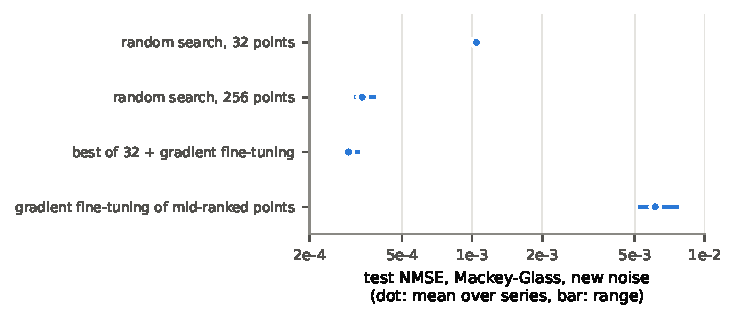
\includegraphics{fig7_gradient}
\caption{Gradient fine-tuning against random search (Mackey--Glass under realistic noise, 512 modes, new noise; dots are means over
three series, bars the range; a range smaller than the marker is hidden). Fine-tuning the best of 32 random points matches extending the random search to 256 points;
fine-tuning points from the middle of the ranking stays far behind the search.}
\label{fig:gradient}
\end{figure}

All twelve fine-tuning runs end better than their starting points, at 0.24 to 0.93 times the starting error, about 0.46 times on
geometric average. The best of 32 random points has $1.04\times10^{-3}$; fine-tuning from it reaches at best $2.9\times10^{-4}$;
extending random search to 256 points directly gives $3.4\times10^{-4}$. The two are comparable, within the spread between noise
realisations. Three further observations limit the role of fine-tuning: the same start with another training seed differs by almost a
factor of two ($2.9\times10^{-4}$ against $5.4\times10^{-4}$); starting from the middle of the ranking, fine-tuning stays above
$6\times10^{-3}$, far worse than the search, so it cannot rescue a mediocre start; and three of the twelve runs were still at their
best at the last validation (step 60), so these had not converged and longer training might help.
In computation random search wins clearly: on the same GPU each fine-tuning run (256 modes, 60 steps) takes about 18~s per step,
about 18 minutes per run and about 2.4 hours for the eight runs from the best four starts, whereas extending random search from 32 to
256 points adds one batched simulation per series (up to 512 operating points per batch, one to two minutes).

At the size of our problem (about 70 real parameters) random search alone is therefore the better choice; gradient fine-tuning is at
most a refinement after the search, and should be run with several training seeds. Differentiable simulation may be more valuable in
two situations: many more tunable quantities (a 64-line mask, or several rings designed together), where random search degrades
quickly while the cost of a gradient barely grows; and objectives with continuous structure that random sampling covers poorly.
Neither was tested here.

\section{Where the limit lies in software terms}\label{sec:software}

So far the software reference has been ``a 31-node ESN with input noise $3\times10^{-3}$ under realistic noise''. The convention refers
the laser intensity noise to the input through the modulation depth (Section~\ref{sec:tasks}), but it strongly affects the conclusion:
in Table~\ref{tab:encodings} the mask ties with the ESN on Mackey--Glass ($3.3\times10^{-4}$ against $3.2\times10^{-4}$), whereas with
input noise $10^{-3}$ the ESN reaches $5.3\times10^{-5}$, about 6 times better than the mask and about 3 times better than the best
single ring with the readout-side changes. This section therefore does not use a single point: it sweeps the software input noise
from 0 to $3\times10^{-3}$ and places the resonator on that curve, answering ``how large and how noisy a software reservoir is one
resonator equivalent to''.

\subsection{Sweeping the software input noise}

Figure~\ref{fig:software} shows the test error of 31-, 100- and 300-node ESNs (and of NG-RC~\cite{gauthier2021} for the closed-loop
task) against input noise, with the same protocol as the resonator (Section~\ref{sec:protocol}); the best resonators of the previous
sections are drawn as horizontal reference lines. The top axis converts input noise to the effective number of bits (ENOB) of an
analog-to-digital converter (ADC): if the full scale spans the input range, $N$-bit quantization noise has an rms of $2^{-N}/\sqrt{12}$, so $10^{-4}$,
$3\times10^{-4}$, $10^{-3}$ and $3\times10^{-3}$ correspond to about 11.5, 9.9, 8.2 and 6.6 bits.

\begin{figure}[htbp]
\centering
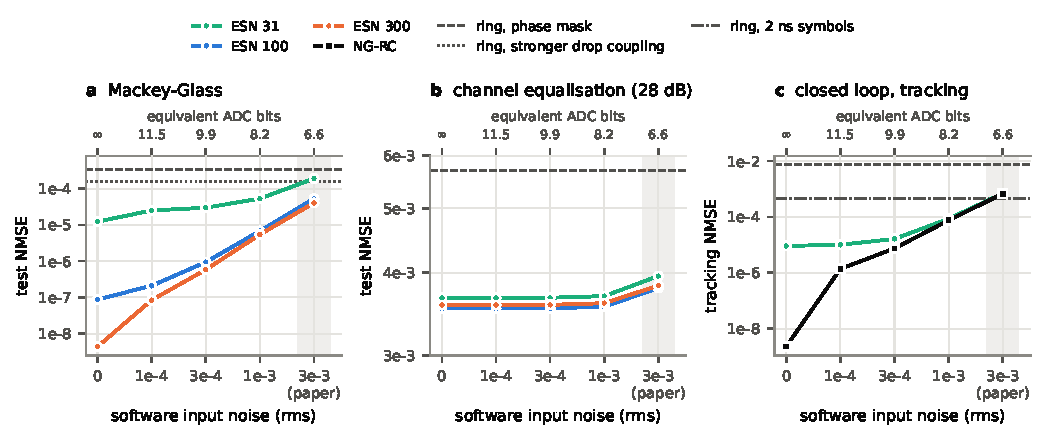
\includegraphics[width=\linewidth]{figS3_esn_input_noise}
\caption{Test error of software reservoirs against their input noise (rms); the top axis gives the equivalent ADC effective bits $N$
(noise $2^{-N}/\sqrt{12}$). Curves: ESNs with 31, 100 and 300 nodes, and NG-RC (closed loop only); horizontal lines: resonators under
realistic noise (plain spectral-phase mask, stronger drop coupling, $2~\mathrm{ns}$ symbols). The grey band marks the convention
$3\times10^{-3}$ used in the previous sections.
(a) Mackey--Glass; (b) channel equalisation (SNR $28~\mathrm{dB}$); (c) closed-loop tracking of a commanded trajectory of the Hénon
map (Appendix~\ref{app:closedloop}). Same selection and re-test protocol as the resonator; Mackey--Glass is the geometric mean over
three series, channel equalisation uses a single series except at $3\times10^{-3}$, and the closed loop averages four training
records.}
\label{fig:software}
\end{figure}

\emph{Mackey--Glass.} The 31-node ESN reaches $1.2\times10^{-5}$, $2.5\times10^{-5}$, $3.0\times10^{-5}$, $5.3\times10^{-5}$ and
$1.9\times10^{-4}$ at input noise 0, $10^{-4}$, $3\times10^{-4}$, $10^{-3}$ and $3\times10^{-3}$; 100- and 300-node ESNs reach
$5.3\times10^{-5}$ and $4.0\times10^{-5}$ at $3\times10^{-3}$, and $8.8\times10^{-8}$ and $4.4\times10^{-9}$ without noise. The best
single ring ($1.55\times10^{-4}$) crosses the 31-node ESN at an input noise of about $2.5\times10^{-3}$; the 100- and 300-node ESNs are
better over the whole sweep, 3 to 4 times at $3\times10^{-3}$.

\emph{Channel equalisation, fibre link and NARMA-10.} The error of the first two tasks comes mostly from the channel's own noise:
lowering the 31-node ESN's input noise from $3\times10^{-3}$ to 0 only moves its error from $3.95\times10^{-3}$ to
$3.66\times10^{-3}$, and growing the ESN to 300 nodes barely matters, but over the whole sweep they beat the best resonator
($5.7\times10^{-3}$); on the fibre link the ESN reaches $1.8\times10^{-2}$ and the best resonator $2.0\times10^{-2}$
(Appendix~\ref{app:fibre}). On NARMA-10 even at $3\times10^{-3}$ the 31-, 100- and 300-node ESNs reach $0.11$, $0.041$ and $0.032$,
better than the single ring's $0.19$.

\emph{Closed-loop decisions.} Appendix~\ref{app:closedloop} uses the resonator to predict the next step of the Hénon map and applies a
bounded control based on the prediction. When tracking a commanded trajectory, the resonator with $2~\mathrm{ns}$ symbols reaches a
tracking error of $4.5\times10^{-4}$ (mean over four training records; $4.4\times10^{-4}$ for the first record shown in
Appendix~\ref{app:closedloop}); the error of the software predictors is set entirely by their input noise and crosses the
resonator at about $2.4\times10^{-3}$, and at $10^{-3}$ the 31-node ESN and NG-RC reach $8.6\times10^{-5}$ and $7.5\times10^{-5}$,
about 5 times better. A second closed-loop task, holding the unstable fixed point of the Hénon map (Appendix~\ref{app:closedloop}), needs only linear
feedback, so the software's modelling capacity is not the limit there, which makes it the cleanest calibration: its crossing is at
about $1.7\times10^{-3}$ (not shown in Fig.~\ref{fig:software}).

The three directly comparable tasks (Mackey--Glass, trajectory tracking and holding the fixed point; on channel equalisation the
curves do not cross) agree: the best single ring matches a 31-node ESN with input noise of about $1.7\times10^{-3}$ to
$2.5\times10^{-3}$, i.e.\ by the conversion above an ADC with about \emph{7 effective bits} (6.9 to 7.4). The ESN curves are medians of
three random reservoirs, and the reservoir-to-reservoir spread (a factor of about 1.7 at $3\times10^{-3}$) moves these crossings by
roughly half a bit. The conversion assumes that the full scale spans the input range $[0,1]$; ENOB as specified for converters refers
to a full-scale sine wave, which differs from this by a fraction of a bit.

\subsection{What 7 bits mean}

This number must be read at the rate at which the resonator works. Our resonator needs $Q\sim10^{6}$ for enough Kerr nonlinearity,
i.e.\ symbol rates of about $0.5$ to $1~\mathrm{GBd}$. Converter resolution falls with sampling rate~\cite{walden1999}; at these rates
off-the-shelf converters offer about 9 effective bits (for
example, a 12-bit converter sampling at $3.2~\mathrm{GSa/s}$ is specified at about 9 effective bits~\cite{ti_adc12dj3200}); converters
with 5 to 6 effective bits are acquisition systems at above $100~\mathrm{GSa/s}$ with tens of gigahertz of bandwidth (for example about
5.9 bits at $33~\mathrm{GHz}$ and 5.0 bits at $110~\mathrm{GHz}$ bandwidth~\cite{keysight_uxr}), and at those rates the resonator's $Q$
can only be $2\times10^{4}$ to $4\times10^{4}$, where the Kerr effect is nearly unused (in the fibre-link task of
Appendix~\ref{app:fibre}, a resonator operated at $28~\mathrm{GBd}$ is only about 15\% better than a linear equaliser). In other
words, at the rates where the resonator works, digitising the signal and handing it to a 31-node software reservoir is no less
accurate than the resonator; a resonator can only be needed where the signal is optical to begin with and digitisation is the very
step to be avoided.

\subsection{The readout must be quantized too}\label{sec:quant}

The software input noise was interpreted above as ADC quantization noise, but the resonator's 31 readings must also be digitised,
and none of the previous results included this step. To make the comparison symmetric we attach one $N$-bit converter to each reading
of the best single ring (Table~\ref{tab:quant}). The full scale of each channel is calibrated once on the run used for fitting and
kept for the test run, i.e.\ the gain is calibrated and then fixed. We consider two front ends: a linear converter digitising the
photocurrent, and a logarithmic amplifier before the converter (equal relative steps, matching the logarithm of the readout). The
reference is a 31-node ESN whose input is quantized to $N$ bits with no other noise, i.e.\ the software side gets a real quantizer
instead of equivalent Gaussian noise.

% generated by experiments/make_table3.py; do not edit by hand
\begin{table}[htbp]
\centering
\caption{Readout quantization. Each of the 31 readings of the best single ring (stronger drop coupling, realistic noise, Mackey--Glass) has its own $N$-bit converter, with the full scale of each channel calibrated once on the fitting run and kept for the test run; ``linear'' digitises the photocurrent, ``log'' places a logarithmic amplifier before the converter. Reference: a 31-node ESN (one random reservoir) whose input is quantized to $N$ bits, with no other noise. Geometric mean over three series $\times$ six new pairs. Unquantized, the resonator reaches $1.5\times10^{-4}$ and the noise-free ESN $2.4\times10^{-5}$.}
\label{tab:quant}
\small
\begin{tabular}{cccc}
\toprule
bits $N$ & resonator, linear & resonator, log amplifier & ESN 31, quantized input \\
\midrule
4 & $4.2\times10^{-3}$ & $1.9\times10^{-3}$ & $3.5\times10^{-3}$ \\
5 & $2.2\times10^{-3}$ & $1.1\times10^{-3}$ & $1.3\times10^{-3}$ \\
6 & $1.2\times10^{-3}$ & $5.6\times10^{-4}$ & $4.5\times10^{-4}$ \\
7 & $6.0\times10^{-4}$ & $3.5\times10^{-4}$ & $2.3\times10^{-4}$ \\
8 & $3.6\times10^{-4}$ & $2.7\times10^{-4}$ & $1.3\times10^{-4}$ \\
9 & $2.7\times10^{-4}$ & $2.1\times10^{-4}$ & $9.3\times10^{-5}$ \\
10 & $2.0\times10^{-4}$ & $1.8\times10^{-4}$ & $6.8\times10^{-5}$ \\
12 & $1.6\times10^{-4}$ & $1.6\times10^{-4}$ & $4.6\times10^{-5}$ \\
\bottomrule
\end{tabular}
\end{table}


The resonator needs many bits not to be degraded by quantization: both front ends need 10 bits to come within 1.3 times of the
unquantized error ($1.54\times10^{-4}$); at 7 bits they reach $6.0\times10^{-4}$ and $3.5\times10^{-4}$, 2 to 4 times worse. The
line powers span several orders of magnitude, so a linear converter gives weak lines few steps; the logarithmic amplifier helps but
does not remove this. At every depth from 6 to 12 bits the ESN with an input quantized to the same depth is 1.2 to 3.4 times better
than the resonator with all 31 channels quantized (against the logarithmic front end; more against the linear one); only at very
coarse quantization, 4 and 5 bits, is the resonator with a logarithmic amplifier better than the ESN, and there both errors are above
$10^{-3}$. Read the other way, the unquantized resonator ($1.54\times10^{-4}$) lies between the ESN with 7- and 8-bit input
quantization ($2.3\times10^{-4}$ and $1.3\times10^{-4}$), consistent with the roughly 7 bits from the equivalent-noise conversion.

Including the readout quantization therefore only makes the comparison less favourable for the resonator: software needs one
converter at its input, the resonator 31, each with about 10 effective bits. Such converters exist at $1~\mathrm{GBd}$, but the power
and cost of 31 channels are a real price. Weighting in the optical domain (computing the readout's linear combination with a spectral
shaper and balanced detection) would need a single converter, but then the delay taps must be implemented with optical delay lines;
we did not simulate such a readout.

\subsection{The limit of ring arrays}

About half of a single ring's error comes from its own detuning jitter and shot noise (Section~\ref{sec:noise}), which are independent
between rings. When several rings with different masks share one input comb and their readouts are concatenated (31 lines $\times$ 8
taps per ring), this part averages out. With 16 times the training length (16\,320 symbols), 1, 2, 4, 8, 16 and 32 rings with stronger
drop coupling reach $1.27\times10^{-4}$, $3.4\times10^{-5}$, $1.36\times10^{-5}$, $8.4\times10^{-6}$, $6.7\times10^{-6}$ and
$6.9\times10^{-6}$: no further gain beyond 16 rings, i.e.\ the error saturates at about 1/19 of a single ring. Letting all rings share
the same laser intensity noise (one input comb split among all rings) barely changes this ($6.8\times10^{-6}$ for 16 rings), so the
saturation does not come from common-mode source noise. With the same training length, ESNs with 100, 300 and 1000 nodes and input noise
$3\times10^{-3}$ reach $3.9\times10^{-5}$, $2.1\times10^{-5}$ and $1.4\times10^{-5}$, so 16 rings are 2 to 6 times better; but with input
noise $10^{-3}$ (one series) they reach $6.8\times10^{-6}$, $3.2\times10^{-6}$ and $1.65\times10^{-6}$: a 100-node ESN already ties with
16 rings and a 1000-node ESN is about 4 times better. An array thus only moves the limit somewhat along the software axis without
changing the conclusion. More rings help only when the task is limited by the rings' own noise: on channel equalisation at
$28~\mathrm{dB}$ channel SNR neither more rings nor a larger ESN helps.

\subsection{Why the $3\times10^{-3}$ convention is strict}

$3\times10^{-3}$ is the laser intensity noise ($10^{-3}$) divided by the modulation depth ($0.33$), which assumes that the software's
input is as noisy as the resonator's. But this source hardly affects the resonator: with only the laser intensity noise on
(Section~\ref{sec:breakdown}) the resonator's error rises only 1.5 to 1.9 times, while the 31-node ESN's error already doubles at input
noise $10^{-4}$. The same intensity noise hurts the resonator far less than it hurts the ESN once referred to the input (possibly
because in the resonator it acts on the pump and all input lines at once and partly appears as a common-mode change; we did not test
this separately). The convention $3\times10^{-3}$ is therefore strict on software, and the statements ``on par with the 31-node ESN''
in the previous sections hold under this strict convention; a fairer point is around $10^{-3}$, where software is better on every task
in this paper.

The conclusion of this section: \emph{within the design space explored and on the tasks studied, the accuracy of a Kerr-microcomb
reservoir stays below that of a software reservoir of the same size; the best single resonator found matches a 31-node ESN fed through
a converter with about 7 effective bits}. This is a statement about one device class (a $200~\mathrm{GHz}$ silica resonator), one
readout (31 drop-port lines, logarithm, linear ridge regression) and one noise model, not a bound for all microcomb reservoirs. The
evaluation protocol is part of it: a single noise realisation is optimistic by 10 to 30\%, results in the chaotic regime are not
reproducible, and the input noise given to software reverses the comparison, so we give whole curves rather than one point.
Section~\ref{sec:bidir} raises the resonator by about one bit with a second set of modes and an optimised mask, against software that
is optimised in the same way.

\section{Discussion}\label{sec:discussion}

\subsection{Experimental implementation}

The ablation (Section~\ref{sec:ablation}) simplifies the implementation considerably: no per-line modulators are needed. A
$200~\mathrm{GHz}$ input comb locked to the resonator FSR is split in two; one branch stays static and the other passes one intensity
or phase modulator carrying the signal. Each branch passes a phase-only (or amplitude-and-phase) spectral shaper that writes the biases
$b_\mu$ and weights $w_\mu$ of Eq.~\eqref{eq:mask}, and the recombined comb enters the resonator with the pump.
Commercial liquid-crystal-on-silicon spectral shapers set the amplitude and phase of each channel independently, with passbands down
to about $10~\mathrm{GHz}$ set in $1~\mathrm{GHz}$ steps, far below the line spacing~\cite{coherent_waveshaper}; C-band models cover
about $5~\mathrm{THz}$ (1527 to $1568~\mathrm{nm}$), enough for 16 input lines ($3.2~\mathrm{THz}$), while 32 lines or more need wider
models; their insertion loss (typically about $5~\mathrm{dB}$, up to 6.5 to $7~\mathrm{dB}$) must be included in the input power
budget. The readout is a demultiplexer after the drop port and 31 photodiodes, the same structure as frequency-multiplexed optical
reservoirs~\cite{butschek2020,lupo2023}. The hardest part is the input comb itself: it must be aligned with the resonator FSR and
phase-stable; we did not simulate its noise.

The requirement on the source follows from Section~\ref{sec:laser}: the intrinsic linewidth of the pump laser relative to the
resonance must be below a few kilohertz. This rules out ordinary DFB lasers ($100~\mathrm{kHz}$ to $1~\mathrm{MHz}$) and calls for a
narrow-linewidth laser or self-injection locking~\cite{shen2020,jin2021}. Slow frequency drift (much longer than one symbol) must be
held by a lock to within about 0.3\% of the half-linewidth; otherwise the trained readout fails as the device drifts (in the
closed-loop experiment of Appendix~\ref{app:closedloop}, a slow drift of 1\% already makes the tracking error 2.4 times worse).

\subsection{Power and rate}

The best single ring needs about $180~\mathrm{mW}$ of total optical input power (stronger drop coupling), and the best points of the
other mask variants lie between about 20 and $200~\mathrm{mW}$; a Si$_3$N$_4$ ring would need about a quarter of that, but then fewer
photons reach the detectors as well, requiring better detectors or an optical amplifier (Section~\ref{sec:platform}). The rate is
limited by the $Q$ needed for the Kerr nonlinearity to about $1~\mathrm{GBd}$. At $1~\mathrm{GBd}$ and $180~\mathrm{mW}$ the optical
energy per symbol is about $180~\mathrm{pJ}$, before the wall-plug efficiency of the laser, the 31 detection channels and the readout
computation. We do not compare energy with digital electronics, because that needs a concrete system scenario, and since the resonator
is not ahead in accuracy (Section~\ref{sec:software}), an energy benefit can only be discussed where the signal is optical and
digitisation can be avoided.

\subsection{Limitations}

\emph{Simulation only.} Our conclusions rest on the LLE and on the noise model. We chose the detector noise from datasheets
($0.3~\mu\mathrm{W}$ per line, in the middle of the 0.13 to $0.63~\mu\mathrm{W}$ of 1-GHz-class InGaAs PIN receivers), the laser
intensity noise and the frequency noise, and checked the latter against realistic spectra; thermorefractive noise of the ring, ASE beat
noise of optical amplifiers, detector quantum efficiency and the noise of the input comb are not modelled. Our implementation of the
literature schemes is also uncertain: the original papers do not give all of the cavity length, the $Q$ split and the sampling
interval, so the comparison should be read as ``in our implementation''.

\emph{Readout.} The readout quantization was computed only for the best single ring and one calibration scheme
(Section~\ref{sec:quant}); a readout weighted in the optical domain was not simulated.

\emph{Tasks.} The three benchmarks and the fibre-link task are standard; the mask's advantage concentrates on prediction that needs strong
nonlinearity and short memory, and tasks with long memory rely on external delay lines (Section~\ref{sec:memory}).

\subsection{Directions that did not work out}

Looking for an advantage of the resonator over software, we tried several more directions, all with negative or limited results. We
summarise them so that others need not repeat them:
\begin{itemize}
\item \emph{Closed-loop decisions} (Appendix~\ref{app:closedloop}): the resonator predicts the Hénon map and a controller acts on the
      prediction. The resonator works in the loop, with decision quality set by the prediction noise; it is slightly ahead of the ESN
      and NG-RC only when the software input noise is $3\times10^{-3}$, and no longer below about $2.4\times10^{-3}$.
\item \emph{A resonator controlling another Kerr resonator}: with a single-mode Kerr cavity as the plant, the resonator controller's
      tracking error ($0.023$) equals that of a 31-node ESN ($0.023$) and of a proportional--derivative controller with feedforward
      ($0.022$), and is only about 3 times better than a plain proportional--derivative controller ($0.068$); when holding the unstable
      state, the proportional--derivative controller and the ESN succeed more often (94\% and 91\%) than the resonator (68\%).
\item \emph{A shared reference ring}: a ring without signal measures the common-mode detuning jitter for subtraction in the readout.
      Even an ideal reference gains only 2\% (Section~\ref{sec:reference}).
\item \emph{Sensing}: the same comb estimates an applied detuning offset (rms error in half-linewidths). Over a narrow range ($\pm0.3$
      half-linewidths) reading 31 lines is only about 1.5 times better than a classical low-power pump-plus-reference reading
      ($1.0\times10^{-3}$ against $1.5\times10^{-3}$); over a wide range ($\pm2$ half-linewidths) the comb is far better than reading the
      pump alone ($0.07$ to $0.09$ against above $0.5$), but a low-power comb with almost no Kerr effect is better still ($0.042$), so the
      benefit comes from probing with many lines, not from the Kerr nonlinearity.
\end{itemize}
These results agree with Section~\ref{sec:software}: in accuracy, what a Kerr-microcomb reservoir can reach is close to a small
software reservoir with quantization noise; its value can only come from the physical layer (an optical signal, latency, energy),
which this paper does not demonstrate and which we leave as an open question.

\section{Conclusion}\label{sec:conclusion}

We used simulations to answer one question: under realistic noise, how good can a Kerr-microcomb reservoir be, what limits it, and how
should it be compared fairly with software.

First, the encoding decides whether the limit can be approached. Giving every line of an input comb a random spectral phase before
modulating it lets the resonator operate in a coherently seeded regime, where the output is set by the input rather than by start-up
noise. Under the same physical conditions and selection budget this spectral-phase mask beats the single-pump encodings of the
literature and a uniformly modulated comb by one to two orders of magnitude on Mackey--Glass prediction, leads slightly on channel
equalisation and does not work on NARMA-10 with a single ring. What matters is the randomness of the line phases, so one modulator and
two spectral phase shapers suffice.

Second, the limit is set by noise, half of it at the source. With ideal detectors about half of the error floor comes from detuning
jitter and half from shot noise; another platform or more power does not lower it, and the readout-side changes (stronger drop
coupling, slower symbols) lower it in part. The jitter cannot be removed in the readout or avoided by another operating point, so the
intrinsic laser linewidth is a hard requirement: below a few kilohertz for our device, while an ordinary $100~\mathrm{kHz}$ laser makes
the error 5 to 6 times worse. The resonator contributes nonlinear features; memory has to come from external delay lines and readout
taps.

Third, in software terms the limit is below software of the same size. The best single ring matches a 31-node ESN fed through a
converter with about 7 effective bits, while at the resonator's rate of about $1~\mathrm{GBd}$ off-the-shelf converters offer about 9;
with the quantization of the resonator's 31 readings included, an ESN quantized only at its input is better at every depth from 6 to 12
bits. Reading several rings together lowers the error another 19 times, but large software reservoirs with lower input noise catch up
as well. The comparison is sensitive to the input noise given to software, so we report whole curves and suggest that future work do
the same.

The value of a Kerr-microcomb reservoir therefore does not lie in computing accuracy and can only come from the physical layer: a signal
that is optical to begin with, digitisation to be avoided, or optical latency and energy. This paper does not demonstrate it; doing so
needs a concrete optical application, an experiment, and a readout weighted in the optical domain that uses a single converter.


\section*{Code and data availability}
The simulator (\texttt{combrc}), all experiment scripts, the result summaries behind every table and figure, and the scripts that
generate them are available under the MIT licence at\\
\url{https://github.com/changxvdu-source/kerr-comb-reservoir}.

\bibliographystyle{unsrtnat}
\bibliography{refs}

\appendix
\section{Numerical checks}\label{app:checks}

\emph{Grid convergence.} Three operating points (Mackey--Glass, first series) were simulated on four grids, 512 or 1024 modes with 20
or 40 RK4IP steps per symbol, each with six new noise realisations; the results agree within the run-to-run spread of about 12\%.
An earlier apparent grid dependence of about 30\% came from the optimistic bias of selecting a point on one noise realisation, not
from the grid. The trained device of Section~\ref{sec:gradient} is the only result where the grid mattered more (14\% between 128 and
256 modes), which is why training uses at least 256 modes and every result is re-checked on 512.

\emph{Selection bias.} Choosing an operating point on one run and reporting the test error of that same run is optimistic by 10 to
30\% at the best points, and sharing one set of noise random numbers across series adds to this. All tables and figures therefore use
the protocol of Section~\ref{sec:protocol}: selection on the mean of three new pairs of runs, reporting on six further new pairs, with
independent noise per series; the software baselines are re-tested in the same way.

\section{Mask ablation}\label{app:ablation}

Figure~\ref{fig:ablation} shows the ablation of Section~\ref{sec:ablation} (realistic noise, 128 random operating points per variant,
the protocol of Section~\ref{sec:protocol}, three series). On both tasks the order is the same: random phases at equal amplitudes are
at least as good as the full mask, random amplitudes in phase are clearly worse, and the uniform comb is worst.

\begin{figure}[htbp]
\centering
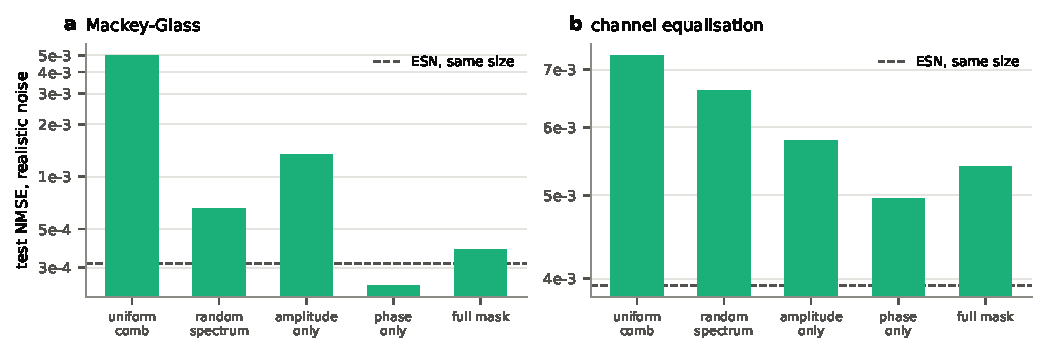
\includegraphics[width=\linewidth]{figS1_mask_ablation}
\caption{Mask ablation under realistic noise. Test error of the uniform comb, a random static spectrum with one common modulation
($w_\mu\propto b_\mu$), random amplitudes with all lines in phase, random phases at equal amplitudes, and the full mask; dashed: ESN
with the same readout dimension (input noise $3\times10^{-3}$). Bars: $\pm1$ relative standard deviation between pairs of new runs
(bars smaller than the marker are hidden).
The full mask gives $3.8\times10^{-4}$ in this batch ($3.3\times10^{-4}$ in Table~\ref{tab:encodings}). (a) Mackey--Glass;
(b) channel equalisation.}
\label{fig:ablation}
\end{figure}

\section{Fibre-link equalisation}\label{app:fibre}

As a realistic communication task we equalise a 28~GBd PAM-4 signal after 17~km of standard single-mode fibre with intensity
modulation and direct detection (chromatic dispersion, loss, Kerr nonlinearity, square-law detection and receiver noise), with 256
random operating points per encoding, the protocol of Section~\ref{sec:protocol} and test parts of 5000 symbols
(Fig.~\ref{fig:fibre}). NMSE and symbol error rate are: $2~\mathrm{ns}$ symbols $2.0\times10^{-2}$ and $1.6\times10^{-3}$; phase mask
$2.3\times10^{-2}$ and $2.3\times10^{-3}$; uniform comb $2.4\times10^{-2}$ and $3.7\times10^{-3}$; best single pump $3.7\times10^{-2}$ and
$1.6\times10^{-2}$; linear equaliser $2.5\times10^{-2}$ and $3.5\times10^{-3}$; ESN $1.8\times10^{-2}$ and $1.4\times10^{-3}$. The bit
error rate of $3.8\times10^{-3}$ commonly used as the hard-decision FEC threshold corresponds, for Gray-coded PAM-4, to a symbol error
rate of about $7.6\times10^{-3}$.
The mask and the readout-side changes beat the linear equaliser and the single-pump encoding but not the ESN (the $2~\mathrm{ns}$ group
is about 15\% worse). These resonators are treated at about 1~GBd, so the comparison is of equalisation capability, not of rate.
Operating the resonator at 28~GBd needs $Q\approx2\times10^{4}$ to $4\times10^{4}$, and with at most 1~W the Kerr effect is barely used:
Si$_3$N$_4$ reaches $2.3\times10^{-2}$ and $2.9\times10^{-3}$, silica $2.4\times10^{-2}$ and $3.2\times10^{-3}$, only about 15\% better than
the linear equaliser in symbol error rate. Without readout taps all encodings are poor here: the memory comes entirely from the taps.

\begin{figure}[htbp]
\centering
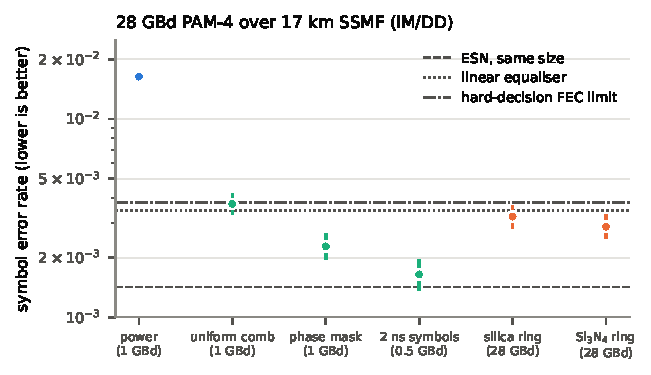
\includegraphics{figS2_fibre_link}
\caption{Symbol error rate on 28~GBd PAM-4 over 17~km of standard single-mode fibre (IM/DD). Blue: single-pump power encoding; green:
input combs processing the received samples offline at 1~GBd or 0.5~GBd (a test of equalisation capability, not of rate); orange:
low-$Q$ rings operated at the link rate (here orange does not denote soliton encodings as in Fig.~\ref{fig:encodings}). Bars: 95\%
Poisson intervals of the error count over 90\,000 symbols. Dashed: ESN with the same readout dimension; dotted: linear equaliser;
dash-dotted: symbol error rate corresponding to the hard-decision FEC threshold (bit error rate $3.8\times10^{-3}$, Gray-coded
PAM-4).}
\label{fig:fibre}
\end{figure}

\section{Closed-loop control}\label{app:closedloop}

The resonator predicts the next state of the Hénon map without control, and a bounded decision rule chooses the control from the
prediction. Two tasks are considered: tracking a commanded trajectory and holding the unstable fixed point. Predictors are compared with
a linear predictor, NG-RC, a 31-node ESN and the exact model; the three resonator variants are each chosen from 64 candidate points and
the ESN from 96.

With PIN detectors the tracking error on the first training record (eight trials, Fig.~\ref{fig:closedloop}b) is $1.0$ for the linear predictor, $7.0\times10^{-4}$ for the ESN,
$6.2\times10^{-3}$ for the plain mask, $2.3\times10^{-3}$ with stronger drop coupling and $4.4\times10^{-4}$ with $2~\mathrm{ns}$ symbols
($2.3\times10^{-5}$ without noise). Holding the unstable fixed point, the $2~\mathrm{ns}$ resonator stays stabilised 99.6\% of the time with
0.4 losses per thousand steps, the same as the exact model; the ESN reaches 99.5\% and 1.6, the plain mask 86\% and 97.
The decision quality is set by the prediction noise: the software predictors' error is set entirely by their input noise
(Fig.~\ref{fig:software}c), and below about $2.4\times10^{-3}$ (tracking) and $1.7\times10^{-3}$ (holding) the ESN and NG-RC are better
than the resonator; at $10^{-3}$ the ESN and NG-RC track with $8.6\times10^{-5}$ and $7.5\times10^{-5}$, about 5 times better.
Detuning jitter with the correlation of the main noise model (one symbol) up to 3\% leaves the $2~\mathrm{ns}$ resonator's tracking error between $4.2\times10^{-4}$ and $5.1\times10^{-4}$
(Fig.~\ref{fig:closedloop}c), but a slow drift (correlation time 1000 symbols) of 1\% makes it 2.4 times worse than the ESN and of 3\%
12 times worse; at 0.1\% and 0.3\% it is still better ($4.2\times10^{-4}$ and $5.6\times10^{-4}$ against $6.9\times10^{-4}$). Slow
detuning drift must therefore be locked to within about 0.3\% of the half-linewidth (about 0.4~MHz at this point). The ranking holds
over four training records with eight trials each (32 trials; mean tracking error of the $2~\mathrm{ns}$ resonator $4.5\times10^{-4}$)
but uses a single textbook map.

\begin{figure}[htbp]
\centering
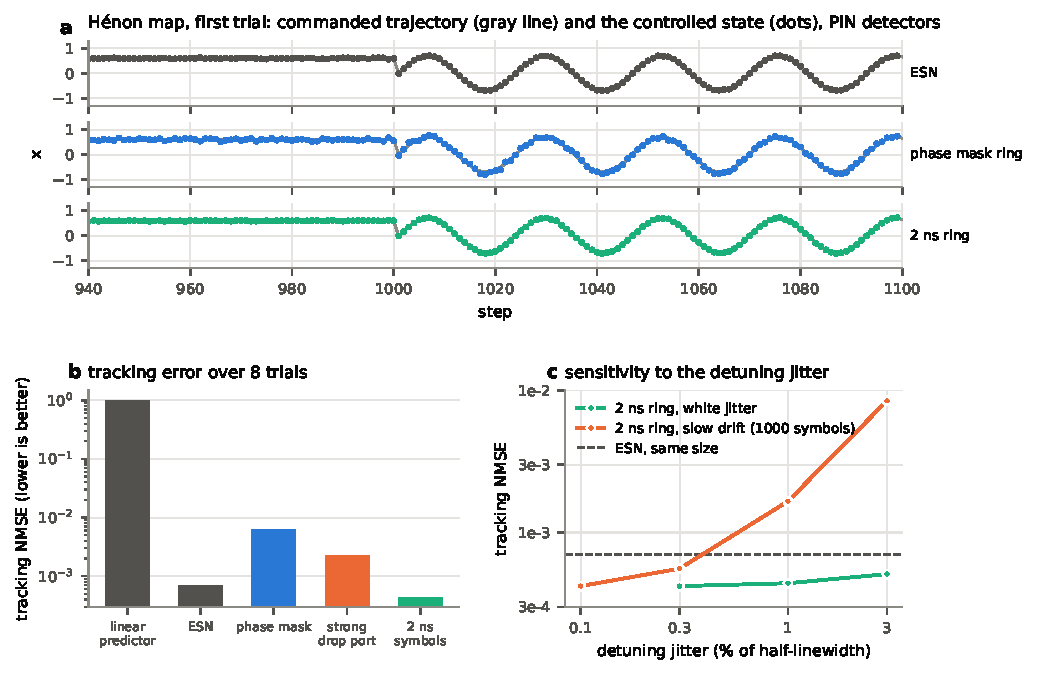
\includegraphics[width=\linewidth]{figS4_closed_loop}
\caption{Closed-loop tracking of the Hénon map with PIN detectors.
(a) First trial: commanded trajectory (grey line) and controlled state (dots) for the ESN, the plain phase-mask resonator and the
resonator with $2~\mathrm{ns}$ symbols. (b) Tracking error, pooled over the eight trials of the first training record (no spread
shown), for the linear predictor, the ESN and three resonator variants. (c) Tracking error of the $2~\mathrm{ns}$ resonator against detuning jitter with a
correlation time of one symbol (as in the main noise model) or a slow drift (correlation time 1000 symbols); dashed: ESN. Software
predictors receive input noise $3\times10^{-3}$ here.}
\label{fig:closedloop}
\end{figure}


\end{document}
